%%% DOCUMENT TYPE %%%%%%%%%%%%%%%%%%%%%%%%%%%%%%%%%%%%%%%%%%%%%%%%%%%%%%%%%%%%%%

\documentclass[11pt, a4paper]{article}

%%% SETUP %%%%%%%%%%%%%%%%%%%%%%%%%%%%%%%%%%%%%%%%%%%%%%%%%%%%%%%%%%%%%%%%%%%%%%

% Analysis

\usepackage{graphicx}
\usepackage{mathtools}
\usepackage{amsfonts} 
\usepackage{fancybox}
\usepackage{textcomp }
\usepackage{bbold}
\usepackage{amssymb}
\usepackage{titlesec}
\usepackage[english,ngerman]{babel}
\usepackage{mathabx} 

\title{Lineare Algebra II}
\author{Frederic Jørgensen}
\date{Erstellt: 01. Februar 2020, Zuletzt ge\aee ndert: \today \\                           % deutsche Ausgabe
	 \selectlanguage{ngerman}}
\pagestyle{headings}
\setlength{\parindent}{0pt}


\newcommand{\sectionbreak}{\clearpage} %Seite bei jedem Abschnitt wechs^{•}eln


%%% PACKAGES %%%%%%%%%%%%%%%%%%%%%%%%%%%%%%%%%%%%%%%%%%%%%%%%%%%%%%%%%%%%%%%%%%%

% Encoding

\usepackage[utf8]{inputenc}
\usepackage[T1]{fontenc}

% Geometry

\usepackage{geometry} % edit margins of paper
\usepackage{setspace} % edit line spacing
\usepackage{fancyhdr} % header, footer
\usepackage{titlesec} % edit format of titles

% Visual

\usepackage[dvipsnames]{xcolor} % colors
\usepackage{tikz} % graphics
\usepackage[framemethod=tikz]{mdframed} % frames, better theorems

% Math

\usepackage{amsmath} % math tools
\usepackage{amssymb} % math symbols
\usepackage{amsthm} % thereoms
\usepackage{mathtools} % math tools

% Referencing

\usepackage{nameref}
\usepackage{hyperref}
\usepackage{cleveref}

% Useful

\usepackage[shortlabels]{enumitem} % enumerations

% Other

\usepackage{lastpage} % get number of last page

%%% MARGINS %%%%%%%%%%%%%%%%%%%%%%%%%%%%%%%%%%%%%%%%%%%%%%%%%%%%%%%%%%%%%%%%%%%%

\geometry{a4paper, left=20mm, right=20mm, top=20mm, bottom=20mm, includehead}

%%% COLORS %%%%%%%%%%%%%%%%%%%%%%%%%%%%%%%%%%%%%%%%%%%%%%%%%%%%%%%%%%%%%%%%%%%%%

%%% COLOR DEFINITIONS %%%%%%%%%%%%%%%%%%%%%%%%%%%%%%%%%%%%%%%%%%%%%%%%%%%%%%%%%%

\colorlet{color-definition}              {Blue!20}%{SpringGreen!20}
\colorlet{color-theorem}                {Brown!25}%{Apricot!13}
\colorlet{color-proposition}            {ProcessBlue!13}% {Apricot!13}
\colorlet{color-corollary}              {Salmon!12}%{Apricot!13}
\colorlet{color-lemma}                  {Brown!7}%{Apricot!13}
\colorlet{color-remark}                 {Gray!4}
\colorlet{color-example}                {Lavender!7}
% \colorlet{color-proof}                  {FILL COLOR HERE}


%%% CAPTIONS %%%%%%%%%%%%%%%%%%%%%%%%%%%%%%%%%%%%%%%%%%%%%%%%%%%%%%%%%%%%%%%%%%%

%%% CAPTION DEFINITION %%%%%%%%%%%%%%%%%%%%%%%%%%%%%%%%%%%%%%%%%%%%%%%%%%%%%%%%%

\newcommand*{\definitionname}{Definition}
\newcommand*{\theoremname}{Theorem}
\newcommand*{\propositionname}{Proposition}
\newcommand*{\corollaryname}{Corollary}
\newcommand*{\lemmaname}{Lemma}
\newcommand*{\remarkname}{Remark}
\newcommand*{\examplename}{Example}


%%% LANGUAGE %%%%%%%%%%%%%%%%%%%%%%%%%%%%%%%%%%%%%%%%%%%%%%%%%%%%%%%%%%%%%%%%%%%

% load language setup (may also include loading packages)

%%% SETUP %%%%%%%%%%%%%%%%%%%%%%%%%%%%%%%%%%%%%%%%%%%%%%%%%%%%%%%%%%%%%%%%%%%%%%

\usepackage[english]{babel}

%%% CAPTION REDEFINITION %%%%%%%%%%%%%%%%%%%%%%%%%%%%%%%%%%%%%%%%%%%%%%%%%%%%%%%



%%% HYPHENATION %%%%%%%%%%%%%%%%%%%%%%%%%%%%%%%%%%%%%%%%%%%%%%%%%%%%%%%%%%%%%%%%



%%% TITLES %%%%%%%%%%%%%%%%%%%%%%%%%%%%%%%%%%%%%%%%%%%%%%%%%%%%%%%%%%%%%%%%%%%%%

\setcounter{secnumdepth}{2}

\titleformat{\section}[block]
{\normalfont\Large\bfseries}{\thesection}{1em}{}
\titleformat{\subsection}[block]
{\normalfont\large\bfseries}{\thesubsection}{1em}{}
\titleformat{\subsubsection}[block]
{\normalfont\normalsize\bfseries}{\thesubsubsection}{1em}{}

\titlespacing*{\section}{0pt}{3.25ex plus 1ex minus .2ex}{2.0ex plus .2ex}
\titlespacing*{\subsection}{0pt}{2.75ex plus 1ex minus .2ex}{1.0ex plus .2ex}
\titlespacing*{\subsubsection}{0pt}{2.25ex plus 0.8ex minus 0.1ex}{0.0ex plus .2ex}

%%% SPACING, LENGTHS, INDENTATION %%%%%%%%%%%%%%%%%%%%%%%%%%%%%%%%%%%%%%%%%%%%%%

\setstretch{1.05} % scaling of space between lines
% \setlength{\topsep}{FILL LENGTH HERE}
% \setlength{\itemsep}{FILL LENGTH HERE}
\setlength{\parskip}{4.0pt plus 1.0pt minus 1.0pt} % space between paragraphs
\setlength{\parindent}{0pt} % indentation of paragraphs

%%% HEADER, FOOTER %%%%%%%%%%%%%%%%%%%%%%%%%%%%%%%%%%%%%%%%%%%%%%%%%%%%%%%%%%%%%

\pagestyle{fancy}
\fancyhf{} % clear everything
\lhead{}
\chead{\large \bfseries \LaTeX{} (Math) Template}
\rhead{Page \thepage /\pageref*{LastPage}}
\lfoot{}
\cfoot{}
\rfoot{}

%%% SHORTCUTS %%%%%%%%%%%%%%%%%%%%%%%%%%%%%%%%%%%%%%%%%%%%%%%%%%%%%%%%%%%%%%%%%%

%%% SINGLE SYMBOLS %%%%%%%%%%%%%%%%%%%%%%%%%%%%%%%%%%%%%%%%%%%%%%%%%%%%%%%%%%%%

% Logic

% \forall exists
% \exists exists
% \lnot exists
% \lor exists
% \land exists
\newcommand*{\limp}{\rightarrow}
\newcommand*{\limps}{\; \limp \;} % \limp with some space around
\newcommand*{\leqv}{\leftrightarrow}
\newcommand*{\leqvs}{\; \leqvs \;} % \leqv with some space around

% Meta Logic

% \implies exists
% \iff exists

% Colon Stuff

\newcommand*{\cl}{\colon}
\newcommand*{\cleq}{\coloneqq}
\newcommand*{\eqcl}{\eqqcolon}

% Sets

\newcommand*{\N}{\mathbb{N}} % natural numbers
\newcommand*{\Z}{\mathbb{Z}} % integers
\newcommand*{\Q}{\mathbb{Q}} % rational numbers
\newcommand*{\R}{\mathbb{R}} % real numbers
\newcommand*{\C}{\mathbb{C}} % complex numbers

%%% MATH OPERATORS %%%%%%%%%%%%%%%%%%%%%%%%%%%%%%%%%%%%%%%%%%%%%%%%%%%%%%%%%%%%%

% General

\DeclareMathOperator{\id}{id}
\DeclareMathOperator{\sgn}{sgn}

%%% TEMPLATES %%%%%%%%%%%%%%%%%%%%%%%%%%%%%%%%%%%%%%%%%%%%%%%%%%%%%%%%%%%%%%%%%%

% General

% write a set definition like: { #1 | #2 }
\newcommand*{\setdefinition}[2]{
  \{#1 \mid #2\}
}

% write a nice map definition
\newcommand*{\mapdefinition}[5]{
  \begin{align*}
    #1 \cl #2 &\to     #3 \\
           #4 &\mapsto #5
  \end{align*}
}


%%% FORMATTING %%%%%%%%%%%%%%%%%%%%%%%%%%%%%%%%%%%%%%%%%%%%%%%%%%%%%%%%%%%%%%%%%

%%% SYMBOLS USED BY NUMBERINGS, ENVIRONMENTS, ... %%%%%%%%%%%%%%%%%%%%%%%%%%%%%%

% \renewcommand*\qedsymbol{$\blacksquare$} % alternative QED symbol
\renewcommand{\thefootnote}{\arabic{footnote}} % normal footnotes on page
\renewcommand{\thempfootnote}{\fnsymbol{mpfootnote}} % footnotes on minipages, e.g. in mdframed environments

%%% MDFRAMED STYLES %%%%%%%%%%%%%%%%%%%%%%%%%%%%%%%%%%%%%%%%%%%%%%%%%%%%%%%%%%%%

% thick frame and bar for title

\mdfdefinestyle{style-box}{
  linewidth=1pt,
  linecolor=Gray!20,
%   roundcorner=3pt,
  innerleftmargin=0.4\baselineskip,
  innerrightmargin=0.2\baselineskip,
  innertopmargin=0.2\baselineskip,
  innerbottommargin=0.2\baselineskip,
  frametitlebackgroundcolor=Gray!20,
  frametitleaboveskip=0.2pt,
  frametitlebelowskip=0.2pt,
  theoremseparator=,
  theoremspace=\hfill,
  theoremtitlefont=\mdseries\scshape,
  nobreak=true
}

% highlighted background

\mdfdefinestyle{style-background}{
  hidealllines=true,
  backgroundcolor=Gray!5,
  innerleftmargin=0.4\baselineskip,
  innerrightmargin=0.2\baselineskip,
  innertopmargin=0.2\baselineskip,
  innerbottommargin=0.2\baselineskip,
}

% thin frame

\mdfdefinestyle{style-thinframe}{
  linewidth=0.4pt,
  linecolor=Gray!30,
  innerleftmargin=0.5\baselineskip,
  innerrightmargin=0.5\baselineskip,
  innertopmargin=0.4\baselineskip,
  innerbottommargin=0.4\baselineskip,
}

%%% ENVIRONMENTS %%%%%%%%%%%%%%%%%%%%%%%%%%%%%%%%%%%%%%%%%%%%%%%%%%%%%%%%%%%%%%%

% Definition

\mdtheorem[
  style=style-box,
  linecolor=color-definition,
  frametitlebackgroundcolor=color-definition
]{definition}{\definitionname}[section]

% Theorem

\mdtheorem[
  style=style-box,
  linecolor=color-theorem,
  frametitlebackgroundcolor=color-theorem,
  font=\itshape
]{theorem}{\theoremname}[section]

% Proposition

\mdtheorem[
  style=style-box,
  linecolor=color-proposition,
  frametitlebackgroundcolor=color-proposition,
  font=\itshape
]{proposition}[theorem]{\propositionname}

% Corollary

\mdtheorem[
  style=style-box,
  linecolor=color-corollary,
  frametitlebackgroundcolor=color-corollary,
  font=\itshape
]{corollary}[theorem]{\corollaryname}

% Lemma

\mdtheorem[
  style=style-box,
  linecolor=color-lemma,
  frametitlebackgroundcolor=color-lemma,
  font=\itshape
]{lemma}[theorem]{\lemmaname}

\theoremstyle{remark}

% Remark

\newtheorem*{remark}{\remarkname}
\surroundwithmdframed[
  style=style-background,
  backgroundcolor=color-remark
]{remark}

% Enumeration Remark

\newenvironment{enumremark}{
  \begin{remark}
    \begin{enumerate}[(a)]
      \item[]
}{
    \end{enumerate}
  \end{remark}
}

% Example

\newtheorem*{example}{\examplename}
\surroundwithmdframed[
  style=style-background,
  backgroundcolor=color-example
]{example}

% Proof

\surroundwithmdframed[
  style=style-thinframe
]{proof}

%%% TEXT FORMATTING %%%%%%%%%%%%%%%%%%%%%%%%%%%%%%%%%%%%%%%%%%%%%%%%%%%%%%%%%%%%

% definitions

\newcommand*{\df}[1]{\colorbox{color-definition}{\emph{#1}}}



%%% DOCUMENT %%%%%%%%%%%%%%%%%%%%%%%%%%%%%%%%%%%%%%%%%%%%%%%%%%%%%%%%%%%%%%%%%%%

%%Todo:
% Definition Integritaetsring


\begin{document}
\maketitle
\tableofcontents
\newpage
\begin{abstract}
	%enterlater
	\centerline{\bt{Stand zum ersten Semester}, Template von Johann Birnick}
\end{abstract}
\section{Eigenwerte}
\subsection{Trigonalisierung}
\begin{definition}
Sei $F : V\ \rightarrow V$ ein Endomorphismus und $W \subset V$ ein Untervektorraum. $W$ heisst $F$-invariant, wenn $F(W) \subset W$.
\end{definition}
\begin{remark}
Ist $W \subset V$ ein $F$-invarianter Unterraum, so ist $P_{F|W}$ ein Teiler von $P_F$.
\end{remark}

\begin{definition}
Eine \bt{Fahne} $(V_r)$ in einem $n$-dimensionalem $V$ ist eine Kette 
\\ \centerline{ $\{0\} = V_0 \subset V_1 \subset ... \subset V_n = V$}
von Untervektorr\aee umen mit $dim V_r = r$. Ist $F \in End(V)$, so heisst die Fahne $F$-invariant, wenn 
\\ \centerline{$F(V_r) \subset V_r$ f\uee r alle $r \in \{0, ... n\}$.}
\end{definition}

\begin{remark}
F\uee r $F \in End(V)$ sind folgende Bedingungen \aee quivalent:
\begin{enumerate}
\item[(i)] Es gibt eine $F$-invariante Fahne in $V$.
\item[(ii)] Es gibt eine Basis $\mathcal{B}$ von V, so dass $M_\mathcal{B}  (F)$ eine obere Dreiecksmatrix ist.
\end{enumerate}
\end{remark}


\begin{theorem} \textbf{(Trigonalisierungssatz)} F\uee r einen Endomorphismus $F$ eines $n$-dimensionalen $K$-Vektorraumes sind folgende Bedingungen \aee quivalent:
\begin{enumerate}
\item[(i)] $F$ ist trigonalisierbar.
\item[(ii)] Das charakteristische Polynom $P_F$ zerf\aee llt in Linearfaktoren.
\end{enumerate}
\end{theorem}

\begin{corollary} Jeder Endomorphismus eines endlich-dimensionalen komplexen Vektorraumes ist trigonalisierbar.
\end{corollary}

\begin{remark} \bt{Rechenverfahren zur Trigonalisierung eines Endomorphismus} von $A \in M(n \times n; K)$
\begin{enumerate}
\item Pr\uee fe, dass $P_A$ in Linearfaktoren zerf\aee llt, aber A nicht diagonalisierbar ist. 
\\
Bestimme einen Eigenvektor $v_1 \in Eig(A, \lambda_1 )$ und erg\aee nze diesen zu einer Basis $\mathcal{B} := (v_1, e_i, ..., e_j)$ des $K^n$. 
\\Betrachte $S^{-1}_1 := T^{\mathcal{B}_1}_{\mathcal{K}}$ und berechne $A_2 = S_1 \cdot A \cdot S_1^{-1} = $
$\left(\begin{array}{ccccc}{
\lambda_{1}} & {*} & {\cdots} & {\cdots} & {*} 
\\ {0} & {\lambda_{2}} & {*} & {\cdots} & {*} 
\\ {\vdots} & {0} & {} & {} 
\\ {\vdots} & {\vdots} & {} & {A_{2}^{\prime}} 
\\ {0} & {0} & {} & {} & {}\end{array}\right)$
\item Bestimme einen Eigenvektor $v_2^{\prime} \in Eig(A_{2}^{\prime}, \lambda_2) $ f\uee r einen Eigenwert $\lambda_2$ von $A_{2}^{\prime}$, erg\aee nze $v_1, v_2$ zu einer Basis $\mathcal{B}_2$ des $K^n$, wobei $v_2$ wie  $v_2^{\prime}$ ist, aber zus\aee tzlich eine 0 als ersten Eintrag hat. Betrachte $S^{-1}_2 := T^{\mathcal{B}_2}_{\mathcal{K}}$ und berechne $A_3 = S_2 \cdot A \cdot S_2^{-1} = $
$\left(\begin{array}{ccccc}{
\lambda_{1}} & {*} & {\cdots} & {\cdots} & {*} 
\\ {0} & {\lambda_{2}} & {*} & {\cdots} & {*} 
\\ {\vdots} & {0} & {} & {} 
\\ {\vdots} & {\vdots} & {} & {A_{3}^{\prime}} 
\\ {0} & {0} & {} & {} & {}\end{array}\right)$

\item Das macht so oft, bis $ D := A_n =S_{n-1} \cdot A \cdot S_{n-1}^{-1}$ eine obere Dreiecksmatrix ist.
\end{enumerate}
\end{remark}
\subsection{Potenzen eines Endomorphismus}
\begin{theorem}
\bt{Satz von Caley-Hamilton} Sei $V$ endlichdimensional und $F \in End(V)$. Dann ist
\\ \centerline{$P_F(F) = 0 \in End(V)$.}
\end{theorem}
\begin{definition}
Eine Teilmenge $\mathcal{I} \subset R$ eines kommutativen Ringes $R$ heisst \bt{Ideal}, wenn gilt:
\begin{enumerate}
\item[I 1] $P, Q \in \mathcal{I} \implies P - Q \in \mathcal{I}$ (Untergruppenkriterium)
\item[I 2] $P \in \mathcal{I}, Q \in R \implies Q \cdot P \in \mathcal{I}$
\end{enumerate}
\end{definition}
\begin{example}
Sei F ein Endomorphismus. Das \bt{Ideal von F} ist definiert als
\\ \centerline{$\mathcal{I}_F := \{ P(t) \in K[t] : P(F) = 0  \} \subset K[t]$.}
\end{example}

\begin{theorem}
Zu jedem Ideal $\mathcal{I} \subset K[t]$ mit $\mathcal{I} \neq \{0\}$ gibt es ein eindeutiges \bt{Minimalpolynom} $M$ mit:
\begin{enumerate}
\item $M$ ist normiert
\item F\uee r jedes $P \in \mathcal{I}$ gibt es ein $Q \in K[t]$ mit $P = Q \cdot M$.
\end{enumerate}
Man nennt das Minimalpolynom von $\mathcal{I}_F$ auch das \bt{Minimalpolynom von F}$M_F$.
\end{theorem}

\begin{theorem}
Sei $n = dim (V)$ und $F \in End(V)$. Dann gilt:
\begin{enumerate}
\item $M_F | P_F$
\item $P_F | M_F^n$
\end{enumerate}
\end{theorem}
%Anderes aus Linalg I ergaenzen?
\begin{definition}
$F \in End(V)$ heisst \bt{nilpotent}, wenn $F^k = 0$ f\uee r ein $k \geq 1$.
\end{definition}
\begin{theorem}
Ist $F \in End(V)$ und $n = dim(V)$. Dann sind folgende Aussagen \aee quivalent:
\begin{itemize}
\item[(i)] $F$ ist nilpotent.
\item[(ii)] $F^d = 0$ f\uee r ein d mit $1 \leq d \leq n$.
\item[(iii)] $P_F = \pm t^n$.
\item[(iv)] Es gibt eine Basis $\mathcal{B}$ von $V$, so dass 
\\ \centerline{
$M_{\mathcal{B}}(F)=\left(\begin{array}{ccc}
{0} & {} & {*} \\ {} & {\ddots} & {} 
\\ {0} & {} & {0}\end{array}\right)$.
}
\end{itemize}
\end{theorem}

\subsection{Die Jordansche Normalform}
\begin{definition}
Sei $F \in End(V)$, so dass $P_F$ in Linearfaktoren zerf\aee llt. Wenn $dim(Eig(F; \lambda_i)) < \mu (P_F; \lambda_i) =: r_i$, kann man die Dimension des Eigenraums vergr\oee ssern: 
\\ \centerline{$Eig(F; \lambda_i) \subset Ker(F - \lambda_i id_v)^{r_i} = Hau(F; \lambda_i)$. }
$Hau(F; \lambda_i)$ nennt man den \bt{Hauptraum} von $F$ zum Eigenwert $\lambda_i$.
\end{definition}
\begin{theorem} \bt{(Satz \uee ber die Hauptraumzerlegung)}
Sei $F \in End_K(V)$, so dass $P_F$ in Linearfaktoren zerf\aee llt. Es sei $V_i := Hau(F, \lambda_i)$ f\uee r alle paarweise verschiedenen Eigenwerte $\lambda_1, ... , \lambda_n \in K$ von $F$. Sei $k := Rg(F)$. Dann gilt:
\begin{enumerate}
\item $F(V_i) \subset V_i$ und $dim(V_i) = \mu (P_F, \lambda_i)$ f\uee r $i = 1, ..., k$. 
\item $V =\bigoplus\limits_{i \in I} V_i$ mit $I=1, ..., k$.
\item $F$ hat eine Zerlegung $F = F_D + F_N$ mit
\begin{enumerate}
\item $F_D$ ist diagonalisierbar
\item$ F_N$ ist nilpotent
\item $F_N$ und $F_D$ kommutieren
\item $F_N$ und $F_D$ lassen sich als Polynome von $F$ schreiben und kommutieren insbesondere mit $F$
\item Wenn man (a), (b) und (c) verlangt, ist diese Zerlegung eindeutig
\end{enumerate}
\end{enumerate}
\end{theorem}

\begin{corollary}
Sei $A \in M(n \times n; K)$, so dass $P_A$ in Linearfaktoren zerf\aee llt. Dann $\exists S \in GL(n)$: 
$$
S A S^{-1}=\left(\begin{array}{cccc}{} & {} & {} & {} 
\\ {\lambda_{1} E_{r_{1}}+N_{1}} & {} & {} & {0} 
\\ {} & {} & {\ddots} & {} 
\\ {0} & {} & {} & {\lambda_{1} E_{r_{1}}+N_{1}} 
\end{array}\right)
$$
wobei f\uee r $i = 1, ... k$
\\ \centerline{$
\lambda_{1} E_{r_{1}}+N_{1} = 
\left(\begin{array}{ccc}
{\lambda_{i}} & {} & {*} 
\\ {} & {\ddots} & {} 
\\ {0} & {} & {\lambda_{i}}\end{array}\right) \in M(r_i \times r_i; K)$.}
mit nilpotenten $N_i$. Insbesondere ist $\tilde{A} = D + N$, wobei $D$ eine Diagonalmatrix und $N$ nilpotent ist und $N$ und $D$ kommutieren.
%%%
\end{corollary}

\begin{lemma}
\bt{(Lemma von Fitting)} Zu einem $G \in End_K(V) $ betrachte
\\ \centerline{$d := min \{ l \in \N : Ker (G^l) =Ker(G^{l + 1}) \}$ und $r := \mu (P_G ; 0)$.}
\\wobei $G^0 := id_V$. Dann gilt:
\begin{enumerate}
\item $d =min \{l : Im(G^l) = Im(G^{l + 1}) \}.$
\item $Ker (G^{d + i}) = Ker (G), \ Im (G^{d + i}) = Im (G^d)\ \forall i \in \N$.
\item Die R\aee ume $U := Ker (G^d)$ und $W := Im (G^d)$ sind $G$-invariant.
\item $(G|U)^d = 0$ und $G|W: W \rightarrow W$ ist ein Isomorphismus.
\item F\uee r das Minimalpolynom von $G|U$ gilt $M_{G|U} = t^d$.
\item $V = U \oplus W$, $dim(U) = r \geq d$, $dim(W) = n - r$.
\\ Insbesondere gibt es eine Basis $\mathcal{B}$ von $V$, so dass
\\ \centerline{$M_\mathcal{B}(G) =
\left(\begin{array}{ll}{N} & {0} 
\\ {0} & {C}\end{array}\right) 
$
mit  $N^d = 0$ und $C \in GL (n-r; K)$.}
\end{enumerate}
\end{lemma}
%to be continued
%Satz seite 256 nochmal aufschreiben
\subsection{Die Normalform von nilpotenten Abbildungen}
\begin{definition}
Die \bt{Jordanmatrix} ist definiert als $J_{k}:=\left(\begin{array}{cccc}
{0} & {1} & {} & {0} 
\\ {} & {\ddots} & {\ddots} & {} 
\\ {} & {} & {\ddots} & {1} 
\\ {0} & {} & {} & {0}\end{array}\right) \in \mathrm{M}(k \times k ; K)$ f\uee r die $J^k = 0$ gilt und $J^{k-1} \neq 0$.
\end{definition}
\begin{theorem}
Sei $G$ ein nilpotenter Endomorphismus eines K-Vektorraums $V$ und $d := min \{l | G^l = 0 \}$. Dann gibt es eindeutig bestimmte Zahlen $s_1, ..., s_d \in \mathbb{N}$ mit 
\\ \centerline{$d \cdot s_d +(d - 1)s_{d-1} + ... + s_l = r = dim V$}
\\und eine Basis $\mathcal{B}$ von $V,$, so dass 
$M_\mathcal{B}(G) =
\left( \begin{array}{cccccccccc}
{J_{d}} & {} & {} & {} & {} & {} & {} & {} & {} & {}
\\ {} & {\ddots} & {} & {} & {} & {} & {} & {} & {0} & {}
\\ {} & {} & {J_{d}} & {} & {} & {} & {} & {} & {} & {}
\\ {} & {} & {} & {J_{d-1}} & {} & {} & {} & {} & {} & {}
\\ {} & {} & {} & {} & {}\ddots & {} & {} & {} & {} & {}
\\ {} & {} & {} & {} & {} & {J_{d-1}} & {} & {} & {} & {}
\\ {} & {} & {} & {} & {} & {} & {\ddots} & {} & {} & {}
\\ {} & {} & {} & {} & {} & {} & {} & {J_{l}} & {} & {}
\\ {} & {0} & {} & {} & {} & {} & {} & {} & {\ddots} & {}
\\ {} & {} & {} & {} & {} & {} & {} & {} & {} & {J_{l}}
\end{array} 
\right)$,
\\wobei $J_d$ $s_d$-mal, $J_{d-1}$ $s_{d-1}$-mal, ... und $J_l$ $s_1$-mal vorkommt.
\end{theorem}

\begin{theorem}
\bt{(Michael-Jordan Normalform)}
Sei $F \in End(V$, wobei das charakteristische Polynom von $F$ in Linearfaktoren zerf\aee llt mit
\\ \centerline{$P_F = \pm (t - \lambda_1)^{r_1} \cdot ... \cdot (t - \lambda_k)^{r_k}$.}
Dann gibt es eine Basis $\mathcal{B}$ von $V$ mit 
$M_\mathcal{B}(F) = 
\left(\begin{array}{ccc}
\lambda_{1} E_{r_{1}}+N_{1} & & 0 
\\ & \ddots &  
\\ 0 & & \lambda_{k} E_{r_{k}}+N_{k}
\end{array}\right).$
\\ $\lambda_i E_{r_i} + N_i = \left(\begin{array}{ccc}
B_{1, d_1} & & 0 
\\ & \ddots &  
\\ 0 & & B_{1, d_2}
\end{array}\right)$
 besteht dabei aus Jordanbl\oee cken, welche diese Form haben:
\\ \centerline{$B_{i, d} = \left(\begin{array}{cccc}\lambda_{i} & 1 & & 
\\ & \ddots & \ddots & 
\\ & & \ddots & 1 
\\ & & & \lambda_{i}\end{array}\right).$}

Ein Jordanblock hat die Gr\oee sse $d$, wenn er d Eintr\aee ge mit $\lambda_i$ und $d - 1$ Einsen oberhalb der Diagonale hat.
Es gilt $1 \leq d_i \leq \mu (M_F, \lambda_i)$ f\uee r $\forall i$.  Der gr\oee sste Jordanblock hat dabei genau die Gr\oee sse $\mu (M_F, \lambda_i)$.

Die Summe der Anzahl der Jordanbl\oee cke multipliziert mit ihrer Gr\oee sse ergibt die algebraische Vielfachheit des Eigenwerts $\lambda_i$.

Man nennt die Elemente $\lambda_i, r_i, d_j$ sowie die Anzahl der Jordanbl\oee cke $s_j^{(i)}$ der Gr\oee sse $d_j$ zum Eigenwert $\lambda_i$ \bt{Invarianten} des Endomorphismus $F$.

Insbesondere ist also die jordansche Normalform ist bis auf die Reihenfolge der Jordanbl\oee cke eindeutig bestimmt.

\textit{Konvention:} Die Jordanbl\oee cke zu einem Eigenwert $\lambda_i$ werden der Gr\oee sse nach absteigend geordnet.
\end{theorem}

\begin{corollary}
$F \in End(V)$ ist genau dann diagonalisierbar, wenn $M_F$ folgende Form hat:
\\ \centerline{$M_F = (t - \lambda_1) \cdot ... \cdot (t - \lambda_k)$,}
wobei $\lambda_1, ... , \lambda_k$ die Eigenwerte von $F$ sind.
\end{corollary}

\begin{remark}
\bt{Rechenverfahren zur Bestimmung einer Jordan-Normalform} von $A \in M(n \times n; K)$
\begin{enumerate}
\item Bestimme die Eigenwerte $\lambda_1, ... \lambda_k$ der Matrix $A$ .
\item Bestimme die Anzahl und Gr\oee sse der Jordanbl\oee cke:

Sei $U = A - \lambda_i E_n$.
Sei $q= min\{l \ | \ dim(Ker(U^l)) = dim(Ker(U^{l+1})\}$ und $s_j^{(i)} = dim(Ker(U^j))$ mit $j \leq q$.
Die Anzahl der Jordanbl\oee cke der Gr\oee sse $j$ zum Eigenwert $\lambda_i$ ist dann gegeben durch 
\\ \centerline{$s_j^{(i)} - s_{j-1}^{(i)} +s_{j+1}^{(i)}.$}
\\
\\
\\ \textit{Kommentar :} Die Anzahl der Jordanbl\oee cke zu $\lambda_i$ ist gegeben durch die geometrische Vielfachheit von $\lambda_i$.
\item Eine jordansche Normalform l\aee sst sich anhand dieser Parameter aufstellen.
\end{enumerate}
\end{remark}

\begin{remark}
\bt{Rechenverfahren zur Bestimmung der Basiswechselmatrix einer Jordan-Normalform} von $A \in M(n \times n; K)$
\begin{enumerate}
\item Bestimme die Eigenwerte $\lambda_1, ... \lambda_k$ der Matrix $A$. Das folgende Verfahren muss f\uee r jeden Eigenwert durchgef\uee hrt werdemn
\item Sei $U = A - \lambda_i E_n$.

Bestimme $Ker(U), ..., Ker(U^q)$ wobei $q= min\{l \ | \ Ker(U^l) = Ker(U^{l+1})\}$. 
\item Bestimme die Gr\oee sse der Jordanbl\oee cke des Eigenwerts $\lambda_i$.
\item F\uee r einen Jordanblock der Gr\oee sse $j$ bestimme einen Vektor $v_j^{(i)} \in Ker(U^q) / Ker(U^{q-1})$ zum Eigenwert $\lambda_i$. Dann ist $v_{k-1}{(i)} = (A - \lambda_i E_n)(v_k) $ f\uee r all $k = 1, ..., j-1.$
\item $\mathcal{B} = (v_1^{(1)}, ..., v_j^{(1)}, ..., v_1^{(k)}, ..., v_j^{(k)})$ ist die gesuchte Basis.

\end{enumerate}
\end{remark}

\section{Euklidische und unit\aee re Vektorr\aee ume}

\subsection{Das kanonische Skalarprodukt im $\mathbb{R}^n$}
\begin{definition}
Das \bt{kanonische Skalarprodukt im $\mathbb{R}^n$} ist die Abbildung $\langle\quad, \quad\rangle: \mathbb{R}^{n} \times \mathbb{R}^{n} \rightarrow \mathbb{R}, \quad(x, y) \mapsto\langle x, y\rangle$ mit $\langle x, y\rangle = x^T \cdot y$.
\\Es hat die folgenden Eigenschaften:
\begin{enumerate}
%Bilinearitaet noch nicht komplett abgeschrieben
\item \bt{Bilinearit\aee t} $\left\langle \alpha x+ \alpha^{\prime} x^{\prime}, y\right\rangle=\alpha \langle x, y\rangle+ \alpha^{\prime}\left\langle x^{\prime}, y\right\rangle $
\\$\left\langle x, \beta y+ \beta^{\prime} y^{\prime}\right\rangle=\beta \langle x, y\rangle+ \beta^{\prime}\left\langle x, y^{\prime}\right\rangle $
\item \bt{Symmetrie} $\left\langle x, y \right\rangle = \left\langle y, x \right\rangle$
\item \bt{Positive Definitheit} $\left\langle x, x \right\rangle \geq 0$ und $\left\langle x, x \right\rangle = 0 \Leftrightarrow x = 0$.
\end{enumerate}
\end{definition}

\begin{definition}
Das \bt{kanonische Skalarprodukt im $\mathbb{C^n}$} ist die Abbildung $\langle\quad, \quad\rangle: \mathbb{C}^{n} \times \mathbb{C}^{n} \rightarrow \mathbb{R}, \quad(x, y) \mapsto\langle x, y\rangle$ mit $\langle x, y\rangle = \overline{x}^T \cdot y$.
\\Es hat folgende Eigenschaften:
\begin{enumerate}
\item \bt{Sesquilinearit\aee t} $\left\langle \alpha x+ \alpha^{\prime} x^{\prime}, y\right\rangle_c=\alpha \langle x, y\rangle+ \alpha^{\prime}\left\langle x^{\prime}, y\right\rangle_c $
\\$\left\langle x, \beta y+ \beta^{\prime} y^{\prime}\right\rangle_c=\overline{\beta} \langle x, y\rangle+ \overline{\beta}^{\prime}\left\langle x, y^{\prime}\right\rangle_c $
\item \bt{Symmetrie} $\left\langle w, z \right\rangle_c = \overline{\left\langle z, w \right\rangle}_c$
\item \bt{Positive Definitheit} $\left\langle z, z \right\rangle \in \mathbb{R}_+$ und $\left\langle z, z\right\rangle_c = 0 \Leftrightarrow z = 0$
\end{enumerate}
\end{definition}

\begin{definition}
Sei $K = \mathbb{R}$ oder $K = \mathbb{C}$. Die \bt{euklidische Norm} ist die Abbildung $\|\cdot\|: K^{n} \rightarrow \mathbb{R}_{+}, \quad x \mapsto\|x\|:=\sqrt{\langle x, x\rangle}$, mit dem kanonischen Skalarprodukt.
\\Dieses erf\uee llt folgende Eigenschaften
\begin{enumerate}
\item $\|x\| \geq 0$ und $\|x\| = 0 \Leftrightarrow x= 0$
\item $ \| \alpha \cdot x \| = \mid\alpha \mid \cdot \|x \| $ 
\item $\|x+y\| \leq\|x\|+\|y\|$
\end{enumerate}
\end{definition}

\begin{definition}
Mit Hilfe von $\langle\quad, \quad\rangle$ definiere \bt{Winkel} wie folgt:
\\Seien $x, y \in \mathbb{R}^n\backslash \{0\} $.
Der Winkel zwischen $x$ und $y$ ist 
\begin{equation*}
\angle(x, y) = \arccos\left(\frac{\langle x, y\rangle}{\|x\| \cdot\|y\|}\right).
\end{equation*}
\end{definition}

\subsection{Bilinearformen und Sesquilinearformen}
%Multilinearform und Bilinearform
\begin{definition}
Seien $V_1, V_2$ Vektor\aee ume und $K$ ein K\oee rper. Eine Abbildung
\begin{equation*}
s : V_1 \times V_2 \rightarrow K
\end{equation*}
heisst \bt{bilinear} falls
\begin{enumerate}
\item[\bt{B1}] $s( \alpha v_1 + \alpha^\prime v_1^\prime, v_2) = \alpha s(v_1, v_2) + \alpha^\prime s(v_1^\prime, v_2)$ und
\item[\bt{B2}] $s(v_1, \beta v_2 + \beta^\prime v_2^\prime) = \beta s(v_1, v_2) + \beta^\prime s(v_1, v_2^\prime)$.
\end{enumerate}
Man nennt einen bilineare Abbildung zus\aee tzlich \bt{symmetrisch}, wenn
\begin{enumerate}
\item[\bt{S}] $s(v, w) = s (w, v)$
\end{enumerate}
und \bt{alternierend}, falls
\begin{enumerate}
\item[\bt{A}] $s(w, v) = - s(v, w)$.
\end{enumerate}
\end{definition}

\begin{definition}
Eine \bt{Multilinearform} 
\begin{equation*}
s : V_1 \times V_2 \times ... \times V_n \rightarrow K
\end{equation*}
ist analog zur Bilinearform definiert, die Bilinearform also ein Spezialfall der Multilinearform.
\\Es gilt also f\uee r alle Koordinaten
\begin{enumerate}
\item[\bt{B1}] $s(v_1, ...,  \alpha v_k + \alpha^\prime v_k^\prime, ...,  v_n) = \alpha s(v_1, ..., v_k, ..., v_n) + \alpha^\prime s(v_1, ..., v_k^\prime, ..., v_n)$.
\end{enumerate}
\end{definition}

\begin{definition}
Eine Abbildung $F \in End(V)$ heisst \bt{semilinear}, falls 
\begin{equation*}
F(v + \lambda w) = F(v ) + \overline{\lambda} F(w) \text{ f"ur } \forall v, w \in V, \lambda \in \mathbb{C}.
\end{equation*}
Man nennt eine Abbildung $s: V \times V \rightarrow \mathcal{C}$ \bt{sesquilinear}, wenn $s$ im ersten Argument linear und im zweiten Element semilinear ist.
$s : V \times V \rightarrow \mathcal{C}$ heisst ausserdem \bt{hermitesch}, wenn gilt
\begin{equation*}
s(v, w) = \overline{s(w, v)}.
\end{equation*}
\end{definition}

\begin{remark} Sei $V$ ein endlich dimensionaler Vektorraum, $s : V \times V \rightarrow K$ eine Bilinearform auf $V$ und $\mathcal{B} = (v_1, ..., v_n)$ eine geordnete Basis von $V$. Seien $v, w \in V$ und $x = \phi^{-1}_\mathcal{B}(v)$, $y = \phi^{-1}_\mathcal{B}(y)$, wobei $\phi^{-1}_B : \mathbb{K}^n \rightarrow V$ das Koordinatensystem von $\mathbb{B}$ ist. Dann ist
\begin{equation*}
s(v, w)= x^T A y=\left(x_{1}, \ldots, x_{n}\right)\left(\begin{array}{ccc}a_{11} & \cdots & a_{1 n} \\ \vdots & & \vdots \\ a_{n 1} & \cdots & a_{n n}\end{array}\right)\left(\begin{array}{c}y_{1} \\ \vdots \\ y_{n}\end{array}\right).
\end{equation*}
Es ist also $(a_{ij}) = s(v_i, v_j)$, wobei $i, j \in \{1, ..., n\}$.
\end{remark}

\begin{theorem}
Sei $V$ ein $n$-dimensionaler endlicher Vektorraum und $\mathcal{B}$ eine Basis von $V$. Dann ist  die Abbildung
\begin{equation*}
s \mapsto M_{\mathcal{B}}(s)
\end{equation*}
von den Bilinearformen auf $M(n \times n; K)$ bijektiv und $s$ genau dann symmetrisch, wenn $M_{\mathcal{B}}(s)$ symmetrisch ist. 
\end{theorem}

\begin{remark}
Ist $\mathcal{A}$ eine Basis von $V$, so ist die Matrix der Sesquilinearform $s : V \times V \rightarrow \mathbb{C}$
\begin{equation*}
A = M_\mathcal{A}(s) = (s(v_i, v_j)).
\end{equation*}
Ist $v = \phi_\mathcal{A}(x), w = \phi_\mathcal{A} (y)$ so ist 
\begin{equation*}
s(v, w) = x^T A \overline{y},
\end{equation*}
wobei $\overline{y}$ die komponentenweise Konjugation ist.
$s$ ist hermetisch genau dann, wenn 
$A= \overline{A}$.
\end{remark}

%eigentlich nicht wichtig da klar
\begin{lemma}
Seien $A, B \in M(n \times n; K)$ mit 
\begin{equation*}
x_TAy = x_TBy = 
\end{equation*}
f\uee r alle $x, y \in K^n$. Dann ist $A = B$. 
\end{lemma}

%11032020
\begin{theorem}\bt{(Transformationformel f"ur Bilinearformen)}
Sei $V$ eine endlichdimensionaler Vektorraum mit Basen $\mathcal{A}$ und $ \mathcal{B}$. F"ur jede Bilinearform $s$ auf $V$ gilt dann
\begin{equation*}
M_\mathcal{B}(s) =( T^\mathcal{B}_\mathcal{A})^T \cdot M_\mathcal{A}(s) \cdot T^\mathcal{B}_\mathcal{A}.
\end{equation*}
Der entscheidende Unterschied ist also $( T^\mathcal{B}_\mathcal{A})^T$ statt $( T^\mathcal{B}_\mathcal{A})^{-1}$.
\end{theorem}

\begin{theorem} \bt{(Transformationsformel f"ur Sesquilinearformen)}
Sei $s : V \times V \rightarrow \mathbb{C}$ eine Sesquilinearform und $\mathcal{A}$ und  $\mathcal{B}$ Basen von $V$. Dann ist
\begin{equation*}
M_\mathcal{B}(s) = {T^\mathcal{B}_\mathcal{A}}^T M_\mathcal{A}(s) \overline{T^\mathcal{B}_\mathcal{A}}
\end{equation*}
\end{theorem}

\begin{definition}
Sei $s: V \times V \rightarrow K$ eine symmetrische Bilinearform. Die \bt{zu $s$ geh"orige quadratische Form} ist die Abbildung
\begin{equation*}
q : V \rightarrow K, v \mapsto s(v, v).
\end{equation*}
Es gilt dann $g(\lambda v) = \lambda^2 q(v)$ f"ur  $\forall v \in V, \lambda \in K$.
Ist $V = K^n$ und $s$ durch die symmetrische Matrix $A = (a_{ij})$ gegeben, gilt:
\begin{equation*}
q(x_1, ..., x_n) = \sum\limits_{i, j = 1}^n a_{ij} x_i x_j = \sum\limits_{j = 1}^n a_ii x_i^2 + 2 \cdot \sum\limits_{1 \leq i < j \leq n} a_{ij}x_ix_j,
\end{equation*}
was ein homogenes quadratisches Polynom in den Unbestimmten $x_1, ..., x_n$ ist.
\end{definition}

\begin{theorem} \bt{(Polarisierung von Bilinearformen)}
Ist $\textrm{char}(K) \neq 2$, so gilt f"ur jede symmetrische Bilinearform $s$ und die zugeh"orige quadratische Form $q$:
\begin{equation*}
s(v, w) = \frac{1}{2}(q(v+w)-q(v)-q(w)) \text{ f"ur } \forall v, w \in V.
\end{equation*}
$s$ ist also aus $q$ konstruierbar.
\end{theorem}

\begin{theorem} \bt{(Polarisierung von Sesquilinearformen)}
Man hat im Komplexen für Sesquilinearformen eine \bt{Polarisierung}
\begin{equation*}
s(v, w)=\frac{1}{4}(q(v+w)-q(v-w)+\mathrm{i} q(v+\mathrm{i} w)-\mathrm{i} q(v-\mathrm{i} w)).
\end{equation*}
\end{theorem}

%richtiges Zeichen ? zwischen UVR und Komplement unterscheiden.
\begin{definition}
Sei $K = \mathbb{R}, \mathbb{C}$ und $V$ eine K-Vektorraum mit einer symmetrischen Bilinearform / hermiteschen Sesquilinearform $s : V \times V \rightarrow K$. 
\\ Dann heisst $s$ \bt{positiv definit}, falls $s(v, v) > 0 \ \forall v \in V/\{0\}$.
Eine solche Bilinearform / Sesquilinearform nennt man auch \bt{Skalarprodukt auf $V$}.
\\$V$ zusammenn mit einem Skalarprodukt nennt man einen \bt{euklidischen Vektorraum} ($K = \mathbb{R})$) bzw. \bt{unit"aren Vektorraum} ($K = \mathbb{C}$).
\\Die \bt{Norm} auf einem euklidischen / unit"aren Vektorraum ist gegeben durch
\begin{equation*}
\\
\| v\| = \sqrt{\left\langle v , v \right\rangle}.
\end{equation*}
\end{definition}

\begin{remark}
Eines symmetrische (bzw. hermitesche) \bt{Matrix} $A \in M( n \times n; K)$ heisst \bt{positiv definit}, falls die zugeh"orige Bilinearform / Sesquilinearform positiv definit ist. 
\end{remark}

\begin{theorem} \bt{(Ungleichung von Cauchy-Schwarz)} Ist $V$ ein euklidischer Vektorraum, gilt f"ur alle $v, w \in V$
\begin{equation*}
|\langle v, w\rangle| \leq\|v\| \cdot\|w\|
\end{equation*}
und Gleichheit genau dann, wenn $v$ und $w$ linear abh"angig sind.
\end{theorem}

\begin{definition}
Definition. Sei \(V\) ein euklidischer bzw. unitärer Vektorraum.
\begin{enumerate}
\item Zwei Vektoren \(v, w \in V\) heißen orthogonal ($v \perp w$), wenn$\langle v, w\rangle= 0.$
\item Zwei Untervektorräume \(U, W \subset V\) heißen orthogonal ($U \perp W$), wenn
\begin{equation*}
u \perp w \text { für alle } u \in U \text { und alle } w \in W \text {. }
\end{equation*}
\item Ist \(U \subset V\) ein Untervektorraum, so definiert man sein orthogonales Komplement
\begin{equation*}
U^{\perp}:=\{v \in V: v \perp u \text { für alle } u \in U\}
\end{equation*}
Das ist wieder ein Untervektorraum.
\item Eine Familie \(\left(v_{1}, \ldots, v_{n}\right)\) in \(V\) heißt orthogonal, wenn
$v_{i} \perp v_{j}$ für alle $ i \neq j.$
\\Sie heißt orthonormal, falls zusätzlich $
\|v_i\| = 1 \text{ f"ur alle } i.
$
\\Sie heisst Orthonormalbasis, falls sie auch eine Basis ist, d.h. eine Basis mit
$\left\langle v_{i}, v_{j}\right\rangle=\delta_{i j} \ \forall i, j.$
%orthogonal zeichen statt oplus
\item Ist \(V=V_{1} \oplus \ldots \oplus V_{k},\) so heißt die direkte Summe orthogonal ($V=V_{1} \obot \ldots \obot V_{k}$), falls
\begin{equation*}
\text { falls } V_{i} \perp V_{j} \quad \text { für alle } i \neq j.
\end{equation*}
\end{enumerate}
\end{definition}

\begin{remark}
Sei $(v_1, ..., v_n)$ eine orthogonale Familie in $V$ mit $v_i \neq 0$ $\forall i$. Dann gilt:
\begin{enumerate}
\item Dann ist 
$$
\left(\frac{1}{\|v_1\|} v_1, \frac{1}{\|v_2\|} v_2, ..., \frac{1}{\|v_n\|} v_n \right)
$$
orthonormal.
\item $(v_1, ..., v_n)$ ist linear unabh"angig.
\end{enumerate}
\end{remark}

\begin{remark}
Sei $(v_1, ..., v_n)$ eine Orthonormalbasis von $V$ und $v \in V$ beliebig. Dann gilt:
$$
v = \left\langle v, v_1 \right\rangle v_1 + ... + \left\langle v, v_n \right\rangle v_n.
$$
\end{remark}

\begin{remark}
Sei $(v_1, ..., v_n)$ eine Orthonormalbasis von $V$ und $v = \lambda_1 v_1 + ... + \lambda_n v_n, \ w =  \mu v_1 + ... + \mu v_n \  \in V$. Dann gilt:
$$
\left\langle v, w \right\rangle = \left\langle \lambda_1 v_1 + ... + \lambda_n v_n, \mu_1 v_1 + ... + \mu_n v_n \right\rangle = \sum\limits_{i = 1}^n \lambda_i \overline{\mu_j} = \left(\begin{array}{ccc}\lambda_1 & \hdots & \lambda_n \end{array} \right) \overline{\left(\begin{array}{c}\mu_1  \\ \vdots \\ \mu_n \end{array} \right)}.
$$
\end{remark}

\subsection{Gram-Schmidtsches Orthogonalisierungsverfahren}
\begin{theorem} \bt{(Orthonormalisierungssatz)}
Sei $V$ ein endlichdimensionaler, euklidischer bzw. unit"arer Vektorraum und $W \subset V$ ein Untervektorraum mit der Orthonormalbasis $(w_1, ..., w_m)$. Dann gibt es eine Erg"anzung zu einer Orthonormalbasis von $V$ $(w_1, ..., w_n, w_{m+1}, ..., w_n)$.
\end{theorem}

\begin{corollary}
Jeder endlichdimensionale Vektorraum hat eine Orthonormalbasis.
\end{corollary}

\begin{corollary}
Sei $W \subset V$ ein Untervektorraum des endlich dimensionalen euklidischen bzw. unit"aren Vektorraumes $V$. Dann gilt
$$
V = W \obot W^\perp \text{ und } dim V = dim W + dim W^\perp.
$$
\end{corollary}

\begin{remark}\bt{(Gram-Schmidtsches Orthogonalisierungsverfahren)}
\begin{enumerate}
\item Erg"anze $(w_1, ..., w_n)$ zu einer Basis $(w_1, ..., w_m, v_{m+1}, ..., v_n)$ von $V$
\item Orthogonalisiere die Basis durch $\tilde{v_i} := v_i - \left( \scp{v_i}{w_1}  w_1 +  ...  + \scp{v_i}{w_m} w_m  \right)$ 
\item Normiere die erhaltenen Vektoren (am Besten f"ur einfachere Rechnung nach jedem Schritt) durch $v_i' = \frac{\tilde{v_i}}{\|\tilde{v_i}\|}.$
\end{enumerate}
\end{remark}

\begin{remark} \bt{(QR-Zerlegung)}
Sei $V = K^n$ und $A \in M(n \times n, K)$. Dann existiert eine Orthogonalmatrix  $Q$ und eine obere Dreiecksmatrix $R$, so dass $$
A = Q \cdot R.$$
\end{remark}

\begin{definition}
Sei $V$ ein unit"arer oder euklidischer Vektorraum und $W \subset V$ ein Untervektorraum mit der Orthonormalbasis $(w_1, ..., w_m)$.
Die \bt{orthogonale Projektion} auf $W$ ist dann der Endomorphismus $P : V \rightarrow W$ gegeben durch 
$$P(v) = \scp{v}{w_1} \cdot w_1 + ... + \scp{v}{w_m}\cdot w_m.$$
\end{definition}
\subsection{Gramsche Determinante und Volumenmessung}

\begin{definition}
Seien $V$ ein euklidischer Vektorraum und $v_1, ..., v_m \in V$, wobei $m \leq n = dim V$.
Dann nennt man 
$$
G\left(v_{1}, \ldots, v_{m}\right):=\operatorname{det}\left(\begin{array}{ccc}\left\langle v_{1}, v_{1}\right\rangle & \cdots & \left\langle v_{1}, v_{m}\right\rangle \\ \vdots & & \vdots \\ \left\langle v_{m}, v_{1}\right\rangle & \cdots & \left\langle v_{m}, v_{m}\right\rangle\end{array}\right) \in \mathbb{R}
$$
die Gramsche Determinante.
\end{definition}

\begin{remark}
Es ist $G\left(v_{1}, \ldots, v_{m}\right) \geq 0$ und es gilt
$$
G\left(v_{1}, \ldots, v_{m}\right) > 0 \Leftrightarrow v_1, ..., v_m \text{ sind linear unabh"angig.}
$$
\end{remark}

\begin{definition}
Das Volumen des von  $v_1, ..., v_m$ aufgespannten Spates ist definiert als 
$$
Vol(v_1, ..., v_m) := \sqrt{G\left(v_{1}, \ldots, v_{m}\right)}.
$$
\end{definition}

\begin{theorem}\bt{(Ungleichung von Hadamard)}
Seien $v_1, ..., v_m \in V$ und $V$ ein euklidischer Vektorraum, wobei $m \leq dim V$. Dann gilt
$$
Vol(v_1, ..., v_m) \leq \|v_1\| \cdot ... \cdot \|v_m\|.
$$
Es besteht Gleichheit genau dann, wenn $v_i \perp v_j$ f"ur $\forall i \neq j$.


\end{theorem}

%18032020
\subsection{Orthogonale und unit"are Endomorphismen}
\begin{definition}
Sei V ein euklidischer / unit"arer Vektorraum und $F \in End(V)$. Dann heisst $F$ orthogonal bzw. unit"ar. falls
$$
\left\langle F(v), F(w) \right\rangle = \left\langle v, w \right\rangle.
$$
\end{definition}

\begin{remark}
Ein orthogonaler / unit"arer Endomorphismus erf"ullt folgende Bedingungen:
\begin{enumerate}
\item $\| F(v) \| = \|v\| \forall v \in W$
\item $ v \perp w \implies F(v) \perp F(w)$
\item $F$ ist ein Isomorphismus und $F^{-1}$ orthogonal bzw. unit"ar
\item Ist $\lambda \in K$ ein Eigenwert von $F$, so gilt $\|\lambda \| = 1$\
\item Die Komposition orthogonaler / unit"arer Endomorphismus ist orthogonal / unit"ar
\end{enumerate}
\end{remark}

\begin{lemma}
Gilt f"ur $F \in End(V)$ dass $\|F(v)\| = \|v\|$ f"ur alle $v \in V$, so ist $F$ orthogonal bzw. unit"ar.
\end{lemma}

\begin{definition}
Eine Matrix $A \in GL(n)$ heisst \bt{orthogonal} bzw. \bt{unit"ar}, falls 
$$
\forall x, y \in K^n: A^{-1} = A^T
\text{ bzw. }
\forall x, y \in K^n :A^{-1} =\overline{A}^T.
$$
$A$ heisst \bt{eigentlich unit"ar}, wenn $\mathrm{det}(A) = 1$.
\end{definition}

\begin{remark}
F"ur eine orthogonale bzw. unit"are Matrix $A$ gilt $|\mathrm{det}(A)| = 1$.
\end{remark}

\begin{definition}
Es sind folgende Untergruppen von $GL(n)$ definiert:
\begin{enumerate}
\item Die orthogonale Gruppe $O(n) = \{ A \in GL(n) | A^{-1} = A^T \}$
\item Die spezielle orthogonale Gruppe $SO(n):=\{A \in O(n): \mathrm{det} A=1\}$
\item Die unit"are Gruppe U(n):=$\{A \in GL(n ; \mathbb{C}): A^{-1}= \overline{A}^T\}$
\item Die spezielle unit"are Gruppe $SU(n):=\{A \in SU(n): \mathrm{det} A=1\}$
\end{enumerate}

\end{definition}

\begin{remark}
Für \(A \in \mathrm{M}(n \times n ; K)\) sind folgende Bedingungen gleichwertig:
\begin{enumerate}
\item \(A\) ist orthogonal bzw. unitär.
\item Die Spalten von \(A\) sind eine Orthonormalbasis von \(K^{n}\).
\item Die Zeilen von \(A\) sind eine Orthonormalbasis von \(K^{n}\).
\end{enumerate}
\end{remark}


\begin{theorem}
Satz. Sei \(V\) ein euklidischer bzw. unitärer Vektorraum mit einer Orthonormalbasis \(\mathcal{B}\) und \(F\) ein Endomorphismus von \(V\). Dann gilt:
$F$ orthogonal bzw. unit"ar $\Leftrightarrow M_{\mathcal{B}}(F)$ orthogonal bzw. unitär.
\end{theorem}

\begin{lemma}
Ist \(A \in O(2),\) so gibt es ein \(\alpha \in[0,2 \pi[,\) so dass
$A=\left(\begin{array}{cc}\cos \alpha  & -\sin \alpha 
\\ \sin \alpha & \cos \alpha\end{array}\right)$ 
oder 
$A=\left(\begin{array}{cc}\cos \alpha & \sin \alpha \\ \sin \alpha & -\cos \alpha\end{array}\right)$.
\end{lemma}

%20032020
\begin{theorem}
Jeder unitäre Endomorphismus \(F\) eines endlich dimensionalen unitären Vektorraumes besitzt
eine Orthonormalbasis aus Eigenvektoren von \(F .\) Insbesondere ist er diagonali-
sierbar.
\end{theorem}

\begin{corollary}
Zu \(A \in U(n)\) gibt es ein \(S \in U(n)\) mit
$$
 \overline{S}^T \cdot A \cdot S = \left(\begin{array}{ccc}\lambda_{1} & & 0 \\ & \ddots & \\ 0 & \lambda_{n}\end{array}\right)
 $$
wobei $\lambda_{i} \in \mathbb{C}$ mit $|\lambda_{i}|=1$ f"ur $i=1, ..., n $.
\end{corollary}


\begin{theorem}
Sei $F$ ein orthogonaler Endomorphismus des endlichdimensionalen euklidischen Vektorraums $V$. Dann gibt es eine Orthonormalbasis $\mathcal{B}$ von $V$, so dass:

$M_\mathcal{B}(F) =
\left( \begin{array}{ccccccccc}
{+1} & {} & {} & {} & {} & {} & {} & {} & {} 
\\ {} & {\ddots} & {} & {} & {} & {} & {} & {0} & {} 
\\ {} & {} & {+1} & {} & {} & {} & {} & {} & {} 
\\ {} & {} & {} & {-1} & {} & {} & {} & {} & {} 
\\ {} & {} & {} & {} & {}\ddots & {} & {} & {} & {} 
\\ {} & {} & {} & {} & {} & {-1} & {} & {} & {} 
\\ {} & {} & {} & {} & {} & {} & {A_1} & {} & {} 
\\ {} & {0} & {} & {} & {} & {} & {} & {\ddots} & {} 
\\ {} & {} & {} & {} & {} & {} & {} & {} & {A_k} 
\end{array} 
\right)$,
wobei $A_{j}=\left(\begin{array}{cc}\cos \vartheta_{j} & -\sin \vartheta_{j} \\ \sin \vartheta_{j} & \cos \vartheta_{j}\end{array}\right) \in SO(2)$ mit $\vartheta_j \in (0, 2\pi), \ \vartheta_j \neq \pi$.

\end{theorem}

\begin{lemma}
Zu einem orthogonalen Endomorphismus \(F\) eines endlichdimensionalen euklidischen Vektorraumes \(V\) mit $dim (V) \geq 1\) gibt es immer einen Untervektorraum \(W \subset V\) mit
$$
F(W) \subset W \text { und } 1 \leq dim (W) \leq 2 .
$$
\end{lemma}



\subsection{Selbstadjungierte Endomorphismen}


\begin{definition}
Der zu einem Endomorphismus $F$ eines euklidischen / unit"aren Vektorraumes $V$ \bt{adjungierte Endomorphismus} $F^{ad} \in End(V)$ ist definiert durch:
$$
\scp{F(v)}{w} = \scp{v}{F^{ad}(w)}
$$
f"ur alle $v, w \in V$.
\end{definition}

\begin{remark}
Sei $\mathcal{B}$ eine Orthonormalbasis von $V$, $F$ ein Endomorphismus und $A = M_\mathcal{B}(F)$. Dann ist der adjungierte Endormorphismus von $F$ eindeutig gegeben durch $M_\mathcal{B}(F^{ad}) = \overline{A}^T$.
\end{remark}

\begin{definition}
Ein Endomorphismus $F$ eines euklidischen / unit"aren Vektorraumes $V$ heisst \bt{selbstadjungiert}, wenn $\scp{F(v)}{w} = \scp{v}{F(w)}$ f"ur alle $v, w \in V$.
\end{definition}

\begin{theorem}
Sei $F$ ein Endomorphismus von \(V\) und \(\mathcal{B}\) eine Orthonormalbasis. Dann gilt: 

\(F\) selbstadjungiert $\Leftrightarrow M_{\mathcal{B}}(F)$ symmetrisch bzw. hermitesch.
\end{theorem}

\begin{lemma}
Die Eigenwerte eines selbstadjungierten Endomorphismus $F \in End(V)$ sind (auch im komplexen Fall) reell. 
\end{lemma}

\begin{theorem}
Ist \(F\) ein selbstadjungierter Endomorphismus eines euklidischen bzw. unitären endlichdimensionalen Vektorraumes, so gibt es eine Orthonormalbasis von \(V\), die aus Eigenvektoren von \(F\) besteht. Insbesondere ist $F$ also diagonalisierbar.
\end{theorem}

\begin{theorem}
Ist \(A \in \mathbb{M}(n \times n ; K)\) eine symmetrische bzw. hermitesche Matrix, so
gibt es eine orthogonale bzw. unitäre Matrix $S$, so dass
$$
\overline{S}^T A S = 
\left(\begin{array}{ccc}\lambda_{1} & & 0 
\\ & \ddots & 
\\ 0 & & \lambda_{n}\end{array}\right)
$$
mit $\lambda_1, ..., \lambda_n \in \mathbb{R}$.
\end{theorem}

\begin{corollary}
Sind \(\lambda_{1}, ..., \lambda_{k}\) die verschiedenen Eigenwerte eines selbstadjungierten oder unitären Endomorphismus \(F\) von \(V\), so ist
$$
V= Eig (F ; \lambda_{1}) \obot ... \obot Eig(F ; \lambda_{k}).
$$
\end{corollary}

\begin{remark} \textit{(Praktische Berechnung einer Orthonormalbasis eines selbstadjungierten Endomorphismus)}
\begin{enumerate}
\item Zerlege $P_F(t) = \pm (t- \lambda_1)^{r_1} ... (t- \lambda_k)^{r_k} $ in Linearfaktoren
\item Bestimme Basen der Eigenr"aume
\item Orthonormalisiere die gefundenen Basen mit dem Gram-Schmidt-Verfahren unabh"angig voneinander in den verschiedenen Eigenr"aumen
\end{enumerate}

\end{remark}

%25032020
\begin{theorem}\bt{(Satz von Courant-Fischer)} Sei $V$ ein endlichdimensionaler euklidischer oder unit"arer Vektorraum und $F \in End(V)$ selbstadjungiert. Seien die Eigenwerte von $F$ 
$$
\lambda_1 \leq ... \leq \lambda_n.
$$
Dann gilt:
\begin{enumerate}
\item $\lambda_k = \min\limits_{U\subset V,\ \mathrm{dim} U = k} \left(   \max\limits_{x\in U\ , \ x \neq 0} \frac{\scp{x}{Fx}}{\scp{x}{x}}\right)$
\item $\lambda_k = \min\limits_{U\subset V,\ \mathrm{dim} U = n - k + 1} \left(   \max\limits_{x\in U\ , \ x \neq 0} \frac{\scp{x}{Fx}}{\scp{x}{x}}\right)$
\end{enumerate}
Die erste Minimierung ist dabei "uber die Untervektorr"aume der angegebenen Dimension.
\end{theorem}
 
\subsection{Hauptachsentransformation und Kriterien f"ur positive Definitheit}

\begin{theorem} \bt{(Hauptachsentransformation)} Sei $A \in M(n \times n; \mathbb{R})$ symmetrisch und $s$ die zugeh"orige Bilinearform, also $s(u, v) = u^T A v$.
\\Dann gilt:
\begin{enumerate}
\item Ist $\mathcal{B} = (w_1, ... w_n)$ eine Orthonormalbasis des $\mathbb{R}^n$, so ist
$$
M_\mathcal{B}(s) = \left(\begin{array}{ccc}\lambda_{1} & & 0 
\\ & \ddots & 
\\ 0 & & \lambda_{n}\end{array}\right), 
$$
wobei $\lambda_1, ..., \lambda_n$ die Eigenwerte von $A$ sind (dies sind Eigenwerte des Endomorphismus $A$, aber nicht der Bilinearform).
\item Es gibt eine Basis $\mathcal{A}$ des $\mathbb{R}^n$, so dass
$$
M_\mathcal{A}(s) =  \left(\begin{array}{ccc}E_k & & 0 
\\ & -E_l & 
\\ 0 & & 0\end{array}\right),
$$
wobei $k$ und $l$ Invarianten der Bilinearform sind (siehe unten).
\end{enumerate}
\end{theorem}

\begin{corollary}
Eine symmetrische Matrix $A \in M(n \times n; \mathbb{R})$ ist genau dann positiv definit, wenn ihre Eigenwerte positiv ist.
\end{corollary}

\begin{corollary}
Eine symmetrische Matrix $A \in M(n \times n; \mathbb{R})$ mit dem charakteristischen Polynom $P_A(t) = (-1)^n t^n + \alpha_{n-1}t^{n-1} + ... + \alpha_0$ ist genau dann positiv definit, wenn $(-1)^j \alpha_j > 0$ f"ur $j = 0, ..., n-1$.
\end{corollary}

\begin{lemma}\bt{(Vorzeichenregel)}
Das reelle Polynom $f(t) = t^n + a_{n-1}t^{n-1} + ... +a_0$ habe die reellen Nullstellen $\lambda_1, ..., \lambda_n$, also $f(t) = (t - \lambda_1) \cdot ... \cdot (t - \lambda_n)$. Dann gilt:
\begin{enumerate}
\item $(\lambda_i < 0 \ \forall i) \Leftrightarrow (a_i > 0 \ \forall i)$
\item $(\lambda_i > 0 \ \forall i) \Leftrightarrow ( (-1)^{n-i}a_i > 0 \ \forall i)$.
\end{enumerate}

\end{lemma}

%27032020
\begin{definition} Sei $s : V \times V \rightarrow \mathbb{R}$ eine symmetrische Bilinearform auf dem endlichdimensionalen $\mathbb{R}$-Vektorraum $V$. Dann ist der \bt{Ausartungsraum} von $s$ 
$$
V_0 = \{ v \in V | s(v, w) = 0 \ \forall w \in V \}.
$$
Der \bt{Rang} von $s$ ist definiert als
$$
rang(s) = dim (V) - dim (V_0).
$$
\end{definition}

\begin{remark} Ist $V = \mathbb{R}^n$ und $A$ die Matrix von einer Bilinearform $s$ auf $V$, so ist $V_0 = Ker(A)$ und $rang(s) = rang(A)$.
\end{remark}

\begin{corollary}
Sei $V$ ein $n$-dimensionaler $\mathbb{R}$-Vektorraum, $s$ eine symmetrische Bilinearform auf $V$ und $r = rang(s)$. Sei $q : V \rightarrow \mathbb{R}$ die zugeh"orige quadratische Form.
Dann gibt es eine Basis $\mathcal{B} = (v_1, ..., v_n)$ von $V$, so dass f"ur v = $\sum\limits_{i=1}^n a_iv_i \in V$ gilt:
$$
q(v) = \sum\limits_{i=1}^k a_i^2 - \sum\limits_{i=k + 11}^r a_i^2.
$$
Man hat insbesondere eine Zerlegung
$$
V = V_+ \oplus V_- \oplus V_0
$$
mit $q(v) > 0 \ \forall v \in V_+ \backslash \{0\}, \ q(v) < 0 \ \forall v \in V_- \backslash \{0\}.$
\end{corollary}

\begin{theorem} \bt{(Tr"agheitssatz von Sylvester)}
Hat man f"ur eine quadratische Form $q$ auf dem $\mathbb{R}$-Vektorraum $V$ zwei Zerlegungen 
$$
r_+(q) : = V = V_+ \oplus V_- \oplus V_0 =  V_+' \oplus V_-' \oplus V_0 '
$$
wie im obigen Korollar so sind $r_+(q) : =  dim V_+ = dim V_+ ', r_-(q) : = \ dim V_- = dim V_-'$. Man nennet $(r_+(q), r_-(q))$ auch die \bt{Signatur} von $q$.
\end{theorem}

\begin{corollary}
Sei $A \in M(n \times n, \mathbb{R})$ symmetrisch und $S \in GL(n, \mathbb{R})$. Dann haben $A$ und $S^T A S$ die gleiche Anzahl positiver und negativer Eigenwerte mit Vielfachheit gez"ahlt.
\end{corollary}

\subsubsection{Bilinearformen "uber allgemeine K"orper}
\begin{theorem}\bt{(Orthogonalisierungssatz)} 
Sei $V$ endlichdimensionaler $K$-Vektorraum mit $char K \neq 2$ und $s : V \times V \rightarrow K$ eine symmetrische Bilinearform. Dann gibt es eine Basis $\mathcal{B} = (v_1, ..., v_n)$ von $V$, so dass
$$
s(v_i, v_j) = 0 \text{ f"ur } i \neq j.
$$
\end{theorem}

\begin{corollary}
Zu einer symmetrischen Matrix $A \in M(n \times n, K)$ gibt es ein $S \in GL(n, K)$, so dass 
$$
S^T A S = \left(\begin{array}{ccc}\alpha_{1} & & 0 
\\ & \ddots & 
\\ 0 & & \alpha_{n}\end{array}\right) = D
$$
diagonal ist.
\end{corollary}

\begin{remark} \bt{(Rechenverfahren zur Bestimmung solcher $S$ und $D$)}
\begin{enumerate}
\item Schreibe $A | E_n$
\item F"uhre an $A$ simultane Zeilen- und Spaltenumformungen ($A$ ist ja symmetrisch) und an $E_n$ nur die entsprechenden Spaltenumformungen durch, bis $A$ Diagonalform hat. Dann ist $D = C_1^T \cdot ... \cdot C_k^T A \cdot C_k \cdot ... \cdot C_1$ und $S = C_k \cdot ... \cdot C_1$.
\\ Dieses Verfahren ist auch effektiv bei der "Uberpr"ufung positiver Definitheit.
\\
\\
Um im Komplexen ein $S \in GL(n, \mathbb{C})$ mit $S^T A \overline{S} = D$ zu finden, suche $T = \overline{S}$ mit $\overline{T}^T A T = D$ und konjugiere bei jeder Zeilenumformung die Koeffizienten.
\end{enumerate}


\end{remark}

\begin{remark}
Ist $g : U \rightarrow K$ die zur Bilinearform $s : V \times V \rightarrow K$ hgeh"orige quadratische Form und $B = (v_1, ... , v_n)$ eine Basis wie im Satz, so folgt mit $a_j := q(v_j)$, dass f"ur $v = x_1 v_1 + ... + x_n v_n \in V$ gilt 
$$
q(v) = q(v_1) x_1^2 + ... + q(v_n) x_n^2 = a_1 x_1^2 + ... + a_n x_n^2,
$$
wobei die Werte der $a_j$ nicht eindeutig durch $s$ festgelegt sind.

\end{remark}

%nicht mehr allgemeine Koerper
\begin{theorem}
Sei $A \in M(n \times n; \mathbb{R})$ symmetrisch und $A_k$ der $k\times k$ Block von $A$ oben links (Hauptminor). Dann ist $A$ genau dann positiv definit, wenn $det(A_k) > 0 \ \forall k = \{1, ..., n\}$.
\end{theorem}

%31032020, Version fuer hermitesche Sesquilinearformen, neben reelken Saetzen einordnen?

\begin{theorem}
Sei $A \in M (n \times n, \mathbb{C} )$ hermitesch. Sei $s$ die entsprechende Sesquilinearform auf $\mathbb{C}^n$. Dann gilt:
\begin{enumerate}
\item Es gibt eine Orthonormalbasis des $\mathbb{C}^n$, so dass 
$$
M_\mathcal{B}(s) = \left(\begin{array}{ccc}\lambda_{1} & & 0 
\\ & \ddots & 
\\ 0 & & \lambda_{n}\end{array}\right), 
$$
wobei $\lambda_1, ..., \lambda_n$ die Eigenwerte von $A$ sind.
\item Es gibt eine Basis $\mathcal{A}$ des $\mathbb{C}^n$, so dass
$$
M_\mathcal{A}(s) =  \left(\begin{array}{ccc}E_k & & 0 
\\ & -E_l & 
\\ 0 & & 0\end{array}\right). 
$$
\item Die Zahlen $k, l$ aus $2.$ sind gerade die Anzahl der positiven und negativen Eigenwerte von $A$. 
\end{enumerate}
\end{theorem}

\begin{theorem}
Sei $A \in M (n \times n, \mathbb{C}$ eine hermitesche Matrix. Dann sind "aquivalent:
\begin{enumerate}
\item A ist positiv definit, also $x^TA\overline{x} > 0$ f"ur alle $x \in \mathbb{C}^n, \ x \neq 0$.
\item Alle Eigenwerte von $A$ sind positiv.
\item Es gibt ein $S \in GL(n, \mathbb{C})$, so dass $S^TA\overline{S}$ diagonal ist mit positiven Diagonaleintr"agen.
\item Es gibt eine Matrix $T \in GL(n, \mathbb{C})$, so dass
$$
A = \overline{T}^T T
$$
\item Sei $P_A(t) = (-t)^n - \alpha_{n-1}t^{n-1} + ... + \alpha_1 t + \alpha_0 \ \in \mathbb{R} [t]$ das charakteristische Polynom von $A$. Dann gilt 
$$
(-1)^j\alpha_j > 0 \text{ f"ur } j = 0, ..., n-1
$$
\item Sei $A_k  \in M(k \times k, \mathbb{C})$ die $k \ times k$ Untermatrix von $A$ "oben links". Dann gikt
$$
\mathrm{det}A_k > 0 \text{ f"ur  } k = 1, ..., n
$$
\end{enumerate}
\end{theorem}

%nacg oben zu Definition positiv definit
\begin{definition}
Man nennt eine Bilinearform / Sesquilinearform \bt{positiv semidefinit}, falls 
$$
s(v,v) \geq 0 \ \forall v \in V, \ v \neq 0.
$$
\\
Man nennt eine Bilinearform / Sesquilinearform \bt{negativ definit}, falls 
$$
s(v,v) < 0 \ \forall  v \in V, \ v \neq 0.
$$
Dies ist "aquivalent zu $-s$ positiv definit.
\\
Man nennt eine Bilinearform / Sesquilinearform \bt{negativ semidefinit}, falls 
$$
s(v,v) \leq 0 \  \forall v \in V, \ v \neq 0.
$$
\end{definition}


\section{Dualit"at und Tensorprodukte}
\subsection{Dualr"aume}
\begin{definition}
Ist $V$ ein $K$-Vektorraum, so heisst $V^* = \mathrm{Hom}_K(V, K)$ Dualraum von $V$. Elemente von $V^*$ heissen Linearformen auf $V$.
\end{definition}
 

\begin{remark}
Sei $\mathcal{B} = (v_1, ..., v_n)$ eine Basis von $V$. Definiere $V_i^*: V \rightarrow K$ so, dass 
$$
V_i^*(v_j) = \delta_{ij}
$$
Dann ist $\mathcal{B}^* = (V^*_1, ..., V^*_n)$ eine Basis von $V^*$, die \bt{duale Basis}.
\end{remark}

\begin{corollary}
Sei $v \in V$ mit $v \neq 0$. Dann gibt es $\varphi \in V^*$, si dass $\varphi (v) \neq 0$.
\end{corollary}

\begin{corollary}
Zu jeder Basis $\mathcal{B} = (v_1, ..., v_n)$ gibt es einen Isomorphismus
$$
\psi_\mathcal{B} :V \rightarrow V^*
$$ 
mit $\psi_\mathcal{B}(v_i) = V^*_i$.
\end{corollary}
 
\begin{definition}
Sei $U \subseteq V$ ein Untervektorraum. Dann heisst der Untervektorraum
$$
U^0 = \{ \varphi \in V^* | \varphi(u) = 0 \ \forall u \in U \} \subset V^*
$$
der zu $U$ \bt{orthogonale Raum} oder \bt{Annulator} von $U$/
\end{definition}

\begin{theorem}
Ist $(u_1, ... u_k)$ eine Basis eines Untervektorraums $U \subset V$ und $(u_1, ... u_k, v_1, ..., v_k)$ eine Basis von $V$, so bilden die Linearformen $(v_1^*, ..., v_k^*)$ eine Basis von $U_0$ und es ist insbesondere 
$$
\mathrm{dim} U_0 = \mathrm{dim} V - \mathrm{dim} U.
$$
\end{theorem}
 

\begin{definition}
Seien $V< W$ Vektorr"aume und $F : V \rightarrow W$ ein lineare Abbildung. Dann ist die zu $F$ duale Abbildung
$$
F^* : W^* \rightarrow V^*
$$
definiert durch
$$
\psi \rightarrow \psi \circ F =: F^*(\psi).
$$
$F^*$ ist wieder linear.
\\Ausserdem ist die Abbildung $\mathrm{Hom}(V, W) \rightarrow \mathrm{Hom} (W^*, V^*)$, $F \rightarrow F^*$ wieder linear.
\end{definition}
 
\begin{theorem}
 Seien $V, W$ Vektorr"aume mit Basen $\mathcal{A}, \mathcal{B}$ und $F : V \rightarrow W$ gegeben. Dann gilt
$$
 M^{B^*}_{A^*}(F^*) = \left(M^{A}_B(F)\right)^T.
$$
\end{theorem}

\begin{theorem}
Sei $F : V \rightarrow W$ linear, dann gilt 
$$
\mathrm{Im}F^* = \left( \mathrm{Ker} F \right)^0, \ \mathrm{Ker}F^* = \left( \mathrm{Im} F \right)^0.
$$
\end{theorem}

\begin{corollary}
Es gilt $\mathrm{Rang}F* = \mathrm{Rang}F$.
\end{corollary}

\begin{definition}
Zu einem Dualraum $V^*$ nennt man den 
\bt{Bidualraum}
$$
V ^{**} = (V^*)^* = Hom(V^*, K).
$$
Man hat eine kanonische Abbildung 
$$
\iota : V \rightarrow V^{**}
v \mapsto \iota_v
$$
mit $\iota_v(\varphi) = \varphi (v)$.
\end{definition}

\begin{theorem}
F"ur jeden endlich dimensionalen Vektorraum $V$ ist die kanonische Abbildung
$$
\iota : V \rightarrow V^{**}
$$
ein Isomorphismus.
\end{theorem}

\begin{corollary}
F"ur jede lineare Abbildung $F : V \rightarrow W$ gilt $F^{**} = F$, sofern man $V$ und $V^{**}$ und $W$ und $W^{**}$ mittels $\iota$ identifiziert. Man kann sich das am besten mit den Darstellungsmatrizen vorstellen: $M^{\mathcal{A}^{**}}_{\mathcal{B}^{**}} = M^\mathcal{A}_\mathcal{B}$.
\end{corollary}

\begin{remark}
F"ur jeden Untervektorraum $W \subset V$ gilt $(W^0)^0$ = W.
\end{remark}

\subsection{Dualit"at und Skalaprodukte}
\begin{definition}
F"ur bilineare Abbildungen $V \times W \rightarrow K$ sind die Abbildungen
$$
b_v : W \rightarrow K, w \mapsto b(v, w)
$$
$$
b_w : V \rightarrow K, v \mapsto b(v, w)
$$
linear. Die Abbildungen $v \mapsto b_v$ und $w \mapsto b_w$ sind ihrerseits linear, so dass man diese linearen Abbildung enerh"alt:
$$
b ' : V \rightarrow W^*, v \mapsto b_v \in W^*
$$
$$
b '' : W \rightarrow V^*, w \mapsto b_w \in V^*.
$$
Eine Bilinearform $b$ heisst \bt{nicht ausgeartet} falls $b'$ und $b''$ injektiv sind.
\end{definition}

\begin{theorem}
Seien $V$ und $W$ endlichdimensionale Vektorr"aume und $B : V \times W \rightarrow K$ eine nicht ausgeartete Bilinearform, so sind die Abbildungen 
$$
b': V \rightarrow W^*, \ b'':W \rightarrow V^*
$$
Isomorphismen.
\end{theorem}

%06042020
\begin{corollary}
In einem euklidischen Vektorraum ist die kanonische Abbildung
$$
\Psi : V \rightarrow V^*, \ 
v \mapsto \scp{v}{-}
$$
ein Isomorphismus.
\end{corollary}

\begin{theorem}
Sei $V$ ein euklidischer Vektorraum, $\Psi : V \rightarrow V^*$ wie oben. Dann gilt:
\begin{enumerate}
\item F"ur jeden Untervektorraum $U \subset V$ ist $\Psi(U^\perp) = U_0$
\item Ist $\mathcal{B} = (v_1, ..., v_n)$ eine Orthonormalbasis von $V$ und $\mathcal{B}^* = (v_1^*, ..., v_n^*)$ eine duale Basis, so ist $\Psi(v_i) = v_i^*$ f"ur $i = 1, ..., n$ also $\Psi = \Psi_\mathcal{B}$.
\end{enumerate}
\end{theorem}

\subsubsection{Adjungierte Abbildungen}
\begin{definition}
Seien $V, W$ euklidische Vektorr"aume und $F : V \rightarrow W$ eine lineare Abbildung. Dann konstruieren wir die adjungierte Abbildung zu $F$
$$
F^{ad} : W \rightarrow V
$$
die eindeutig bestimmt ist durch
$$
\scp{F(v)}{w} = \scp{v}{F^{ad}(w)}.
$$
\end{definition}

\begin{remark}
Seien $\Phi$ und $\Psi$ die kanonischen Isomorphismen f"ur $V$ und $W$. Dann heisst das, dass $F^{ad} = 
\Phi^{-1} \circ F^{*} \circ \Psi$.
Dieses Diagramm kommutiert also:
\begin{xy}
  \xymatrix{
      W \ar[r]^{F^{ad}} \ar[d]_{\Psi}   &   V \ar[d]^\Phi  \\
      W^* \ar[r]_{F^*}             &   V^*   
  }
\end{xy}

\end{remark}

\begin{remark}
Sind $V, W$ euklidische Vektorr"aume mit Orthonormalbasis $\mathcal{A}$ und $\mathcal{B}$, so gilt f"ur jede lineare Abbildung $F : V \rightarrow W$
$$
M_\mathcal{A}^\mathcal{B}(F^{ad}) = \left( M_\mathcal{A}^\mathcal{B}(F)\right)^T.
$$
\end{remark}

\begin{theorem}
Seien $V, W$ euklidische Vektorr"aume und $F : V \rightarrow W$ linear, so gilt
%durch orthogonales summenzeichen ersetzen
$$
\mathrm{Im}(F^{ad}) = (\mathrm{Ker}F)^\perp
$$
und
 $$
\mathrm{Ker}(F^{ad}) = (\mathrm{Im}F)^\perp.
$$
Insbesondere hat man orthogonale Zerlegungen
$$
V = \mathrm{Ker} F \obot \mathrm{Im}F^{ad}
$$
$$
W = \mathrm{Ker}F^{ad} \obot \mathrm{Im}
$$
Ist $V = W$ und $F$ selbstadjungiert gilt
$$
V = \mathrm{Ker}F \obot \mathrm{Im}F.
$$

\end{theorem}

\subsection{"Ubertragung auf unit"are Vektorr"aume}
\begin{definition}
Sei $V$ ein $\mathbb{C}$-Vektorraum und $s : V \times V \rightarrow \mathbb{C}$ sesquilinear.
Dann hat man eine Abbildung 
$$
s'' : V \rightarrow V^*, \ v \mapsto s(-, v).
$$
, die semilinear ist.

Ist $s$ ein Skalarprodukt erh"alt man den kanonischen Semi-Ismomorphismus (bijektive, semilineare Abbildung)
$$
\Psi : V \rightarrow V^*, v \mapsto \langle - , v \rangle.
$$

Ist $W$ ein unit"arer Vektorraum und $F : V \rightarrow W$ linear, ist die adjungierte Abbildung definiert als 

$$
F^{ad} = \Psi^{-1}_V \circ F^* \circ \Psi_W  : W \rightarrow V.
$$
linear, da zwei semilineare verkn"upft werden.
Aber $ F \mapsto F^{ad}$ ist semilinear.
Es gilt $\langle F(v), w \rangle = \scp{v}{F^{ad}(w)}$.

Der wichtigste Fall ist $V = W$.
\end{definition}

\begin{theorem}
Sei $F \in End(V)$, $V$ ein unit"arer Vektorraum und $F^{ad} \in End(V)$ der adjuntierte Endomorphismus. Dann gilt:
\begin{enumerate}
\item $\scp{F(v)}{w} = \scp{v}{F^{ad}(w)}$
\item $\mathrm{Im}F^{ad} = (\mathrm{Ker})^\perp$ und $\mathrm{Ker}F^{ad} = (\mathrm{Im}F)^\perp$
\item Ist $\mathcal{B}$ eine Orthonormalbasis von $V$ so ist
$$
M_{\mathcal{B}}(F^{ad}) = \overline{M_\mathcal{B}(F)}^T
$$  
\end{enumerate}
\end{theorem}

\begin{remark}
Sowohl im reellen als auch im komplexen Fall gilt 
$$
(F^{ad})^{ad} = F.
$$
Insbesondere gilt auch $\scp{v}{F(w)} = \scp{F^{ad}(v)}{w}.$
\end{remark}


\subsection{Spektralsatz f"ur normale Endomorphismen}

\begin{definition}
Sei $V$ ein unit"arer Vektorraum, $F \in End(V)$. Dann heisst $F$ \bt{normal}, wenn 
$$
F^{ad}\circ F = F \circ F^{ad}.
$$
Entsprechend heisst $A \in M(n \times n, \mathbb{C})$ normal, falls
$$
A \overline{A}^T = \overline{A}^T A.
$$
\end{definition}

\begin{theorem}
Sei $V$ ein unit"arer $\mathbb{C}$-Vektorraum. Dann sind f"ur $F \in End(V)$ "auivalent:
\begin{enumerate}
\item Es gibt eine Orthonormalbasis von $V$ aus Eigenvektoren von $F$.
\item $F$ ist normal.
\end{enumerate}
\end{theorem}

\begin{theorem}
Ist $V$ unit"ar und $F \in End(v)$ normal, so gilt
$$
\mathrm{Ker}F^{ad} = \mathrm{Ker}F \land \mathrm{Im}F^{ad} = \mathrm{Im}F.
$$
Insbesondere ist $V = \mathrm{Ker}F \obot \mathrm{Im}F$.
\end{theorem}

\begin{corollary}
Ist $F$ normal, so ist $\mathrm{Eig}(F, \lambda) = \mathrm{Eig}(F^{ad}, \overline{\lambda})$ f"ur jedes $\lambda \in \mathbb{C}$.
\end{corollary}

\begin{corollary}
Ein $A \in M (n \times nn, \mathbb{C})$ ist genau dann normal, wenn es ein $S \in U(n)$ gibt, so dass $SAS^{-1}$ diagonal ist.
\end{corollary}


%22042020

\subsection{Tensorprodukte}
%siehe auch Beweis fuer konkrete Definition

%Diagramm seite 353 hinzufuegen


\begin{theorem}
Seien $V, W$ $K$-Vektorr"aume. Dann gibt es einen $K$-Vektorraum $V \otimes_K W$ und eine bilineare Abbildung 
$$
\eta: V \times W \rightarrow V \otimes_K W
$$
mit folgender universeller Eigenschaft: Sei $U$ ein $K$-Vektorraum zusammen mit einer bilinearen Abbildung $\xi: V \times W \rightarrow U$. Dann gibt es genau eine lineare Abbildung $\xi_\otimes: V \otimes W \rightarrow U$ so dass $\xi = \xi\otimes_K \circ \eta$.

\begin{gather*}
  \xymatrix{V \times W  \ar[d]|{\eta} \ar[r]|{\xi} & U\\
    V \otimes W \ar[ur]|{\xi_\otimes} & }
\end{gather*}

$V \otimes_K W$ nennt man das \bt{Tensorprodukt} von $V$ und $W$ "uber $K$.

Die Elemente heissen \bt{Tensoren}

Ist ferner $\mathrm{dim}V, \mathrm{dim}W M \infty$ gilt
$$
\mathrm{dim}V \otimes_K W = \mathrm{dim}V \mathrm{dim}W
$$
\end{theorem}


\begin{remark}
Der Vektorraum $V \otimes W$ ist durch die universelle Eigenschaft eindeutig bis auf eindeutigen Isomorphismus bestimmt. 
\end{remark}

\begin{remark}
Seien $(v_i)_{i \in I}, (w_j)_{j \in j}$ Basen von $v$ und $W$.
$V \otimes W$ ist der Vektorraum der endlichen Linearkombinationen formaler Ausdr"ucke der Form $v_i \otimes w_j$:
$V \otimes W := \{ \tau:  I \times J \rightarrow K : \tau(i, j) \neq 0 \text{ f"ur nur endlich viele } (i, j) \in I \times J \}$.
Es ist also $\tau \in V \otimes W$ gegeben durch 
$$
\tau = \sum\limits_{i, j} ' \tau(i, j) (v_i \otimes w_j),
$$
wobei der $'$ bedeutet, dass die Summer nur endlich viele Glieder hat.
Ein Tensor $v_i \otimes w_j \in V \otimes W$ ist also eine Abbildung die nur f"ur $i, j$ $1$ ist und sonst $0$.

Die bilineare Abbildung $\xi$ ist eindeutig gegeben durch $\xi(v_i, w_j) = v_i \otimes w_j$.
Die lineare Abbildung aus der universellen Eigenschaft $\xi_\otimes$ ist nun auch eindeutig bestimmt durch 
$$
\xi_\otimes(v_i \otimes w_j) = \xi(v_i, v_j).
$$
\end{remark}

\begin{remark} (Rechenregeln f"ur Tensoren)
Sei $\eta: V \times W \rightarrow V \otimes W$ und $v \otimes w = \eta(v,w)$ f"ur $v \in V$, $w \in W$. Dann gilt, dass $v \otimes w$ bilinear ist.
\end{remark}

%Komplexifizierung reinschreiben?
\begin{example}
Sei $s : V \times W \rightarrow K$ eine Bilinearform. Schreibe $Bil(V, W; K)$ f"ur den Vektorraum solcher bilinearer Abbildungen, also $s \in Bil(V, W; K)$.
Wir erhalten die lineare Abbildung 
$$
s_\otimes: V \otimes W \rightarrow K, \ s(v \otimes w) = s(v, w)
$$
also $s_\otimes \in (V \otimes W)^*$. 

Die Abbildung 
$$
Bil(V, W; K) \rightarrow (V \otimes W)^*
$$
$$
s \mapsto s_\otimes
$$
ist wieder linear.

Sei umgekehrt $\varphi \in (V \otimes W)^*$, dann ist $\varphi \circ \eta \in Bil(V, W; K)$, wobei $\eta: V \times W \rightarrow V \otimes W$ die bilineare Abbildung aus obigem Satz ist.

Die Abbildungen $s \mapsto s_\otimes$ und $ \varphi \mapsto \varphi \circ \eta $
sind zueinander invers.
\end{example}

\begin{theorem}
Seien $V$ und $W$ $K$-Vektorr"aume. Dann $(V \otimes W)^* \cong Bil(V, W; K)$
\end{theorem}

\begin{example}
Seien $V$ und $W$ Vektorr"aume.
Seien $\varphi \in V^*$, $\Psi \in W^*$ Linearformen.
Dann ist 
$$
\varphi \cdot \Psi: V \times W \rightarrow K
$$
$$
(v, w) \mapsto \varphi (v) \Psi(w)
$$
bilinear.

Wir erhalten eine lineare Abbildung
$$
(\varphi \Psi)_\otimes : V \otimes W \rightarrow K
$$
$$
v \otimes w \mapsto \varphi (v) \Psi(w)
$$
Die erhaltene Abbildung
$$
V^* \times W^* \rightarrow (V \otimes W)^*
$$
$$
(\varphi, Psi) \mapsto (\varphi \Psi)_\otimes
$$
ist bilinear.
Daher erhalten wir eine lineare Abbildung
$$
\alpha: V^* \otimes W^* \rightarrow (V \otimes W)^*
$$
so dass $\varphi \otimes \Psi \mapsto (\varphi \Psi)_\otimes$.

\end{example}


\begin{theorem}
Sind $V$, $W$ endlich dimensional, so ist die Abbildung $\alpha$ von oben ein Isomorphimus, also 
$$
V^* \otimes W^* \cong (V \otimes W)^*.
$$
\end{theorem}

\begin{example}
Wir erhalten eine bilineare Abbildung durch 
$$
V^* \times W \rightarrow \mathrm{Hom}(V,W)
$$
$$
(\varphi, w) \mapsto \varphi (-) \cdot w
$$
mit  $ (\varphi (-) \cdot w) (v) := \varphi (v) \cdot w$.
Wir erhalten eine lineare Abbildung 
$$
\beta: V^* \otimes W \rightarrow \mathrm{Hom}(V, W)
$$
$$
\varphi \otimes w \mapsto \varphi (-) \cdot w
$$
\end{example}

\begin{theorem}
Sind $V$ und $W$ endlich dimensional, so ist die obige Abbildung $\beta:V^* \otimes W \rightarrow \mathrm{Hom}(V, W)$ vom obigen Beispiel ein Isomorphimus. 
\end{theorem}

%24042020
\subsubsection{Tensoren und Matrizen}
Sei $u \in K^m \otimes K^n$, also $u = \sum\limits_{i, j} u_{ij} e_i \otimes e_j$.
Die Koordinaten $u_{ij}$ kann man auf 3 Weisen aufschreiben:
\begin{itemize}
\item Als Matrix $(u_{ij})_{ij} \in M(m \times n, K)$
\item Als $m \cdot n$-Vektor, wobei man die Basis von $K^m \otimes K^n$ wie folgt ordnet:
$\left(\begin{array}{c}
u_{11} \\
u_{21} \\
\vdots \\
u_{m1} \\
\vdots \\
u_{1n} \\
\vdots \\
u_{mn}
\end{array}\right)
$
\item Als $m \cdot  n$ Vektor, wobei man die Basis von $K^m \otimes K^n$ wie folgt ordnet: 
$\left(\begin{array}{c}
u_{11} \\
u_{12} \\
\vdots \\
u_{1n} \\
\vdots \\
u_{m1} \\
\vdots \\
u_{mn}
\end{array}\right)
$
\end{itemize}

\subsubsection{Symmetrisches und "ausseres Produkt}
\begin{definition}
seien $V, W$ Vektorr"aume.
Eine bilineare Abbildung 
$
\xi : V \times V \rightarrow W
$
heisst 
\begin{itemize}
\item symmetrisch, falls $\xi( v, v') = \xi (v', v) \forall v, v' \in V$
\item alternierend, falls $\xi (v, v) = 0 \forall v \in V$. Daraus folgt $\xi(v, v') = - \xi(v' ,v)$. Falls  $\mathrm{char}(K) = 2$ gilt  sogar die Umkehrung.
\end{itemize}
\end{definition}
\begin{lemma}
Wir betrachten die Untervektorr"aume 
$$
S(v) = \mathrm{span} (v \otimes v' - v' \otimes v)_{v, v' \in V} \subset V \otimes V
$$
$$
A(v) =  \mathrm{span} (v \otimes v)_{v \in V} \subset V \otimes V
$$


$\xi : V \times V \rightarrow W$ (bilinear) ist 
\begin{itemize}
\item $\xi$ symmetrisch $\Leftrightarrow S(v) \subset \mathrm{Ker}(\xi_\otimes)$
\item $\xi$ alternierend $\Leftrightarrow A(v) \subset \mathrm{Ker}(\xi_\otimes)$
\end{itemize}
\end{lemma}


\begin{theorem}
F"ur jeden $K$-Vektorraum $V$ mit $\mathrm{dim} V \geq 2$ gibt es einen $K$-Vektorraum $V \wedge V$ zusammen mit einer alternierenden bilinearen Abbildung 
$$\wedge: V \times V \mapsto V \wedge V$$ mit folgender universeller Eigenschaft:

Zu jeder bilinearen alternierenden Abbildung $\xi: V \times V \rightarrow W$ existiert genau eine lineare Abbildung $\xi_\wedge$ so dass
\begin{gather*}
  \xymatrix{V \times V  \ar[d]|{\wedge} \ar[r]|{\xi} & W\\
    V \wedge V \ar[ur]|{\xi_\wedge} & }
\end{gather*}
kommutiert.
Ist $(v_1, ..., v_n)$ eine Basis von $V$, so ist $(v_i \wedge v_j) = \wedge(v_i, v_j)$ mit $q \leq i < j \leq n$ eine Basis von $V \wedge V$. Insbesondere 
$$
\mathrm{dim}(V \wedge V) = \left(\begin{array}{c} n\\ 2 
\end{array} \right) = \frac{n(n-1)}{2}.
$$
\end{theorem}
$V \wedge V = V \otimes V / A(V)$, $\wedge = \rho \circ \eta$ mit der kanonischen Abbildung des Quotientenraums $\rho: V \otimes W \rightarrow V \wedge V$ und der kanonischen Abbildung $\eta: V \times V \rightarrow V \otimes V$.


\begin{remark}(Rechenregeln f"ur das "aussere Produkt.
F"ur $v, v', w, w' \in V$ und $\lambda \in K$ gilt
\begin{itemize}
\item $(v + \lambda v') \wedge w = v  \wedge w + \lambda(v'  \wedge w )$
\item $v  \wedge (w + \lambda w') = v  \wedge w + \lambda(v  \wedge w ')$
\item $v \wedge v = 0$ und $ v \wedge v' = - v' \wedge v$
\end{itemize}
\end{remark}

\begin{theorem}
Man definiert analog das symmetrische Produkt:

Zu jedem $K$-Vektorraum $V$ gibt es einen $K$-Vektorraum $V \vee V$ und eine symmetrische bilineare Abbildung $\vee: V \times V \rightarrow V \vee V$ mit der universellen Eigenschaft:

Sei $\xi : V \times V \rightarrow W$ symmetrisch (und bilinear), dann gibt es genau eine lineare Abbildung $\xi_V: V \vee V \rightarrow W$, so dass
\begin{gather*}
  \xymatrix{V \times V  \ar[d]|{\vee} \ar[r]|{\xi} & W\\
    V \vee V \ar[ur]|{\xi_\vee} & }
\end{gather*}
kommutiert.

Ist $(v_1, ..., v_n)$ eine Basis von $V$, so bilden die Vektoren

$v_i \vee v_j = \vee (v_i, v_j)$ mit $q \leq i \leq j \leq n$ eine Basis von $V \vee V$. Insbesondere
$$
\mathrm{dim}(V \vee V) = \left(\begin{array}{c} n+1\\ 2 
\end{array} \right) = \frac{n(n+1)}{2}.
$$
$V \vee V$ heisst 2. symmetrische Potenz / symmetrischer Produktraum von $V$.
\end{theorem}

Sei nun $\mathrm{Bil}(V; W)$ der Vektorraum der bilinearen Abbildungen $V \times V \rightarrow W$ und $\mathrm{Alt}^2(V, W) \subset \mathrm{Bil}(V; W)$ der Untervektorraum der alternierenden Bilinearformen und $\mathrm{Sym}^2 \subset \mathrm{Bil}(V; W)$ der Untervektorraum der symmetrischen Bilinearformen.

Dann haben wir folgende Abbildungen 
\\
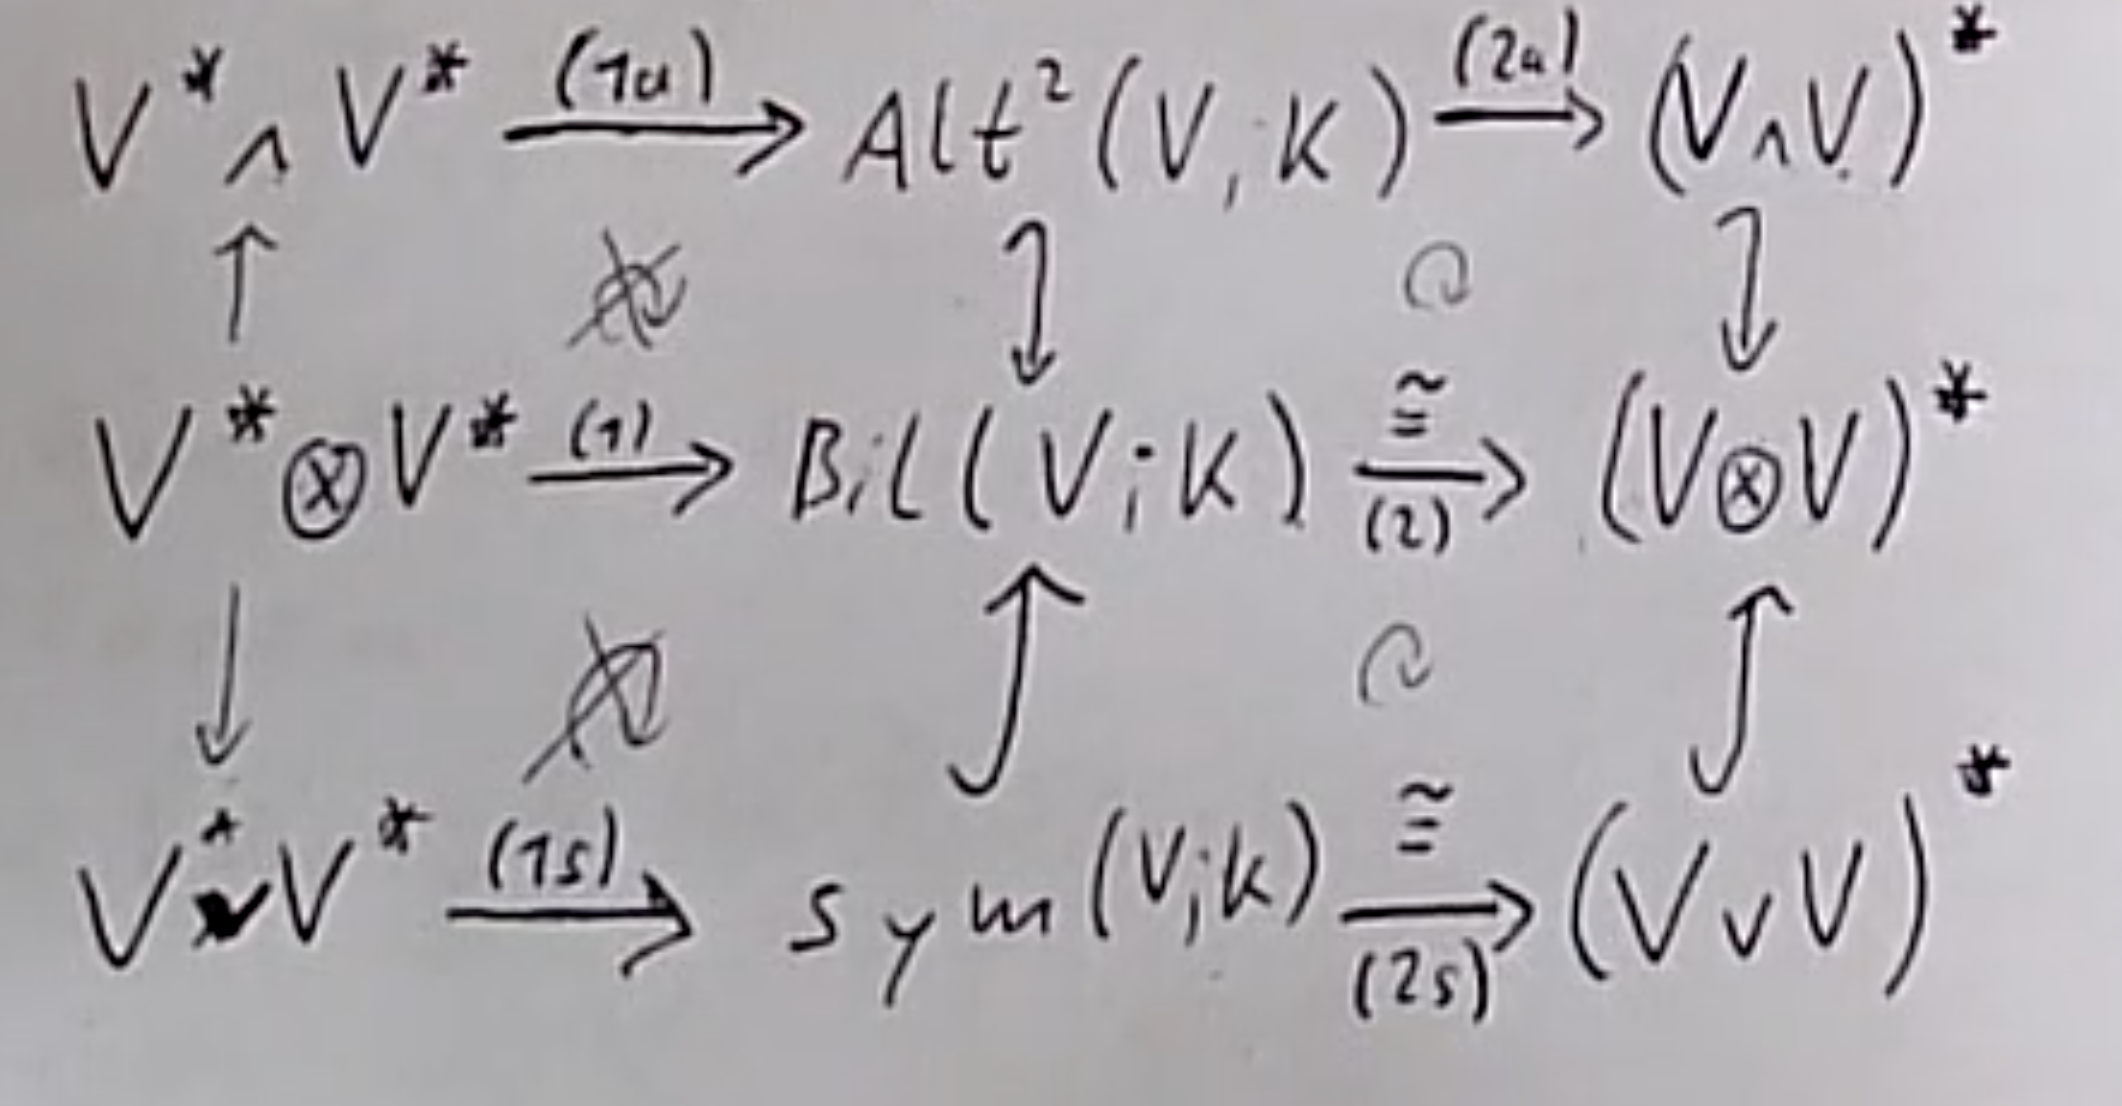
\includegraphics[scale=0.4]{Diagramm}
\\
%Diagramm noch in Latex erstellen
%$$
%\begin{array}{l}\text { Alt }^{2}(V ; K) \subset \operatorname{Bil}(V ; K) \\ \quad \downarrow \\ (V \wedge V)^{*} \quad \subset(V \otimes V)^{*}\end{array}
%$$
\begin{enumerate}
\item Die Abbildungen $(2a)$ und $(2a)$ erhalten wir genau wie $(2)$ aus den universellen Eigenschaften.
\item Die Abbildung $(1a)$ ist definiert durch 
$$
(1a): V^* \wedge V^* \rightarrow \mathrm{Alt}^2(V;K)
$$
$$
(\varphi, \Psi) \mapsto \alpha (\varphi, \Psi) = 
\alpha(\varphi, \psi)(v, w):=\operatorname{det}\left(\begin{array}{cc}\varphi(v) & \varphi(w) \\ \psi(v) & \psi(w)\end{array}\right)
$$
\item Die Abbildung $(1s)$ ist
$$
(1s): V^* \vee V^* \rightarrow \mathrm{Sym}^2 (V;K)
$$
$$
(\varphi, \Psi) \mapsto \operatorname{det}\left(\begin{array}{cc}\varphi(v) & - \varphi(w) \\ \psi(v) & \psi(w)\end{array}\right)
$$
\end{enumerate}

\begin{theorem}
Ist $\mathrm{dim}V < \infty$, so ist $(1a)$ ein Isomorphismus und falls zus"atzlich $\mathrm{char}K = 2$, so ist $(1s)$ auch ein Isomorphismus.
\end{theorem}

\subsection{Multilineare Algebra}
\begin{remark}
Eine multilineare Abbildung ist eindeutig durch die Bilder der Kombinationen der Basisvektoren von den Vektorr"aumen auf denen sie definiert ist bestimmt.
\end{remark}

\begin{definition}
Eine Abbildung zwischen Vektorr"aumen heisst multilinear, wenn sie in jedem Argument linear ist. 
\end{definition}

\begin{theorem}
Zu $K$-Vektorräumen $(V_1,...,V_k)$ gibt es genau einen $K$-Vektorraum $(V_1  \otimes ...  \otimes V_k)$ zusammen mit einer universellen multilinearen Abbildung 
$$
\eta : V_1 \times ... \times V_k  \rightarrow V_1\otimes ... \otimes V_k ,   (v_1,...,v_k) \mapsto v_1\otimes...\otimes v_k
$$
d.h. zu jeder multilinearen Abblidung
$$
\xi: V_1 \times ... \times V_k \rightarrow W
$$
gibt es genau eine lineare Abbildung $\xi_\otimes$ derart, dass das Diagramm 
\begin{gather*}
  \xymatrix{(V_1 \times ... \times V_k)  \ar[d]|{\eta} \ar[r]|{\xi} & W\\
    (V_1 \otimes ... \otimes V_k) \ar[ur]|{\xi_\otimes} & }
\end{gather*}
kommutiert. Sind alle $V_j$ endlichdimensional mit Basen 
$$
(v_1^{(1)},...,v_{rj}^{(k)}), j = 1,...,k,
$$
so ist eine Basis von $(V_1  \otimes ...  \otimes V_k)$ gegeben durch
$$
(v_{i1}^{(1)} \otimes...\otimes v_{ik}^{(k)}) \textit{ mit }  1 \leq i_j \leq r_j)
$$ 
Insbesondere ist $\mathrm{dim}(V_1\otimes...\otimes V_k) = \mathrm{dim} V_1\cdot ... \cdot \mathrm{dim}V_k$
\end{theorem}

\begin{remark}
Es gilt $V_1 \otimes ... \otimes V_k $% Isomorphien hinschreiben
\end{remark}

%Bemerkung Spezialfall Tensoren Physik mit Dualraeumen, Kovarianz / Kontravarianz
\begin{remark}
Ein wichtiger Spezialfall in der Physik ist f"ur einen endlich dimensionalen Vektorraum $V$
$$
T:= \otimes^p V^* \otimes^q V.
$$
Ein Element aus $T$ nennt man $p$-fach kovariant und $q$-fach kontravariant. Man schreibt f"ur eine Basis von $V$ $\mathcal{A} = (v_1, ..., v_n)$ und f"ur die duale Basis $\mathcal{A}^* = (v^1, ..., v^n)$.
%Reihenfolge Transformationsmatrix korrekt? Steht A oder B unten?
Die Begriffe kovariant und kovariant berufen sich auf das unterschiedliche Transformationsverhalten unter Basiswechseln. Sei $\mathcal{B} = (w_1, ..., w_n)$ eine weitere Basis von $V$ und $(a_ij)_{i, j} = T^\mathcal{B}$. Dann gilt
$$
v_i =\sum\limits_{j = 1}^n a_{ji}w_j.
$$
Wegen $T^{\mathcal{A}^*}_{\mathcal{B}^*} = (T^{\mathcal{A}}_{\mathcal{B}})^{-T}$ ist 
$$
v_i^* =\sum\limits_{j = 1}^n \tilde{a_{ij}}w_j^*.
$$
\end{remark}

\begin{definition}
Sind $V$ Und $W$ Vektorräume über $K$, so heißt eine $k$-fach linerare Abblidung
$$
\xi: V^k \rightarrow W
$$
\begin{itemize}
\item  \emph{symmetrisch}, wenn $\xi(v_1,...,v_k) = \xi(v_{\sigma(1)},...v_{\sigma(k)})$ für jede Permutation $\sigma \in S_k$,
\item \emph{alternierend}, wenn $\xi(v_1,...,v_k) = 0 $, falls $ v_i = v_j$ für ein Paar $(i,j)$ mit $i \neq j$
\end{itemize}
\end{definition}

\begin{remark}
Ist $\xi$ alternierend und $ \sigma  \in S_k$, so ist
$$ 
\xi(v_{\sigma(1)},...v_{\sigma(k)}) = \textit{sign}(\sigma) \cdot \xi(v_1,...,v_k)
$$
F"ur $\mathrm{char}K \neq 2$ gilt auch die R"uckrichtung.
\end{remark}

\begin{lemma}
In $\otimes^k$ betrachten wir Untervektorräume 
$$ 
S^k(V) = \mathrm{span} (v_1 \otimes... \otimes v_k  - v_{\sigma(1)},...v_{\sigma(k)})_{v_1 \otimes... \otimes v_k \in  \otimes^k V} \subset \otimes^k V
$$
$$ A^k(V) = \mathrm{span} (v_1 \otimes... \otimes v_k) \subset \otimes^k V, \textit{ wobei  } v_i = v_j \textit{ für ein (i,j) mit  } i\neq j 
$$
Für jedes $k$-fach lineare $\xi: V^k \rightarrow W$ gilt:
\begin{itemize}
\item $\xi$ symmetrisch $\Leftrightarrow S^k(v) \subset \mathrm{Ker}(\xi_\otimes)$
\item $\xi$ alternierend $\Leftrightarrow A^k(v) \subset \mathrm{Ker}(\xi_\otimes)$
\end{itemize}

\end{lemma}

\begin{theorem}
Zu $K$-Verktorräumen und einer natürlichen Zahl $k \geq 1$ gibt es einen $K$-Vektorraum
$\wedge^k$  zusammen mit einer universellen alternierenden Abbildung 
$$
\wedge: V^k \rightarrow \wedge ^k W
$$
d.h. zu jeder alternierenden Abbildung 
$$
\xi: V^k \rightarrow W
$$
gibt es genau eine lineare Abbildung $\xi_{\wedge}$ derart, daß das Diagramm 
\begin{gather*}
  \xymatrix{V^k   \ar[d]|{\wedge} \ar[r]|{\xi} & W\\
    \wedge^k V \ar[ur]|{\xi_\wedge} & }
\end{gather*}

kommutiert. Ist $(v_1,...,v_n)$ eine Basis von $V$, so ist eine Basis von $\wedge^k V$ gegeben durch die Produkte 
$$
v_{i_1} \wedge ... \wedge v_{i_k} \text{ mit } 1 \leq i_1 < ... <  i_k \leq n
$$
Insbesodere ist $\mathrm{dim}\wedge^k = \binom{n}{k}$ für $ 1 \leq k \leq n = \mathrm{dim}V$. Für $k>n$ setzt man 
$$
\wedge^k = 0.
$$


\end{theorem}

\begin{theorem}
Zu $K$-Verktorräumen und einer natürlichen Zahl $k \leq 1$ gibt es einen $K$-Vektorraum
$\wedge^k$  zusammen mit einer symmetrsischen Abbildung 
$$
\vee: V^k \rightarrow \wedge ^k W
$$
so dass f"ur jede symmetrische Abbildung 
$$
\xi: V^k \rightarrow W
$$
genau eine lineare Abbildung $\xi_{\vee}$ existiert derart, daß das Diagramm 
\begin{gather*}
\xymatrix{V^k   \ar[d]|{\vee} \ar[r]|{\xi} & W\\
\vee^k V \ar[ur]|{\xi_\vee} & }
\end{gather*}

kommutiert. Ist $(v_1,...,v_n)$ eine Basis von $V$, so ist eine Basis von $\vee^k V$ gegeben durch die Produkte 
$$
v_{i_1} \vee ... \vee v_{i_k} : =  \vee (v_{i_1}, ..., v_{i_k}) \text{ mit } 1 \leq i_1 \leq ... \leq  i_k \leq n
$$
Insbesodere ist $\mathrm{dim}\vee^k = \binom{n+k-1}{k}$ für $ 1 \leq k \leq n = \mathrm{dim}V$. 
\end{theorem}


\begin{definition}
Seien $V, V', W, W'$ Vektorr"aume und $F \in \mathrm{Hom}(V, V')$, $G \in \mathrm{Hom}(W, W')$. Dann definiert man das Tensorprodukt dieser Abbildungen folgendermassen als lineare Abbildung
$$
F \otimes G: V \otimes W \rightarrow V' \otimes W',
$$
so dass $(F \otimes G)(v \otimes w) = F(v) \otimes G(v)$ f"ur alle $v\in V, w \in W$.
\end{definition}
%Isomorphe Eigenschaft hinzufuegen? 

\begin{theorem}
F"ur endlichdimensionale Vektorr"aume $V, V', W, W'$ ust das Tensorprodukt von Abbildungen 
$$
\otimes: \mathrm{Hom}(V, V') \otimes  \mathrm{Hom}(W, W') \rightarrow \mathrm{Hom}(V \otimes W, V' \otimes W')
$$
ein Vektorraumisomorphismus.
\end{theorem}


 
\section{N\uee tzliche Formeln und Hinweise}

\end{document}
